%% 
%% Copyright 2007-2019 Elsevier Ltd
%% 
%% This file is part of the 'Elsarticle Bundle'.
%% ---------------------------------------------
%% 
%% It may be distributed under the conditions of the LaTeX Project Public
%% License, either version 1.2 of this license or (at your option) any
%% later version.  The latest version of this license is in
%%    http://www.latex-project.org/lppl.txt
%% and version 1.2 or later is part of all distributions of LaTeX
%% version 1999/12/01 or later.
%% 
%% The list of all files belonging to the 'Elsarticle Bundle' is
%% given in the file `manifest.txt'.
%% 

%% Template article for Elsevier's document class `elsarticle'
%% with numbered style bibliographic references
%% SP 2008/03/01
%%
%% 
%%
%% $Id: elsarticle-template-num.tex 168 2019-02-25 07:15:41Z apu.v $
%%
%%
\documentclass[preprint,12pt]{elsarticle}

%% Use the option review to obtain double line spacing
%% \documentclass[authoryear,preprint,review,12pt]{elsarticle}

%% Use the options 1p,twocolumn; 3p; 3p,twocolumn; 5p; or 5p,twocolumn
%% for a journal layout:
%% \documentclass[final,1p,times]{elsarticle}
%% \documentclass[final,1p,times,twocolumn]{elsarticle}
%% \documentclass[final,3p,times]{elsarticle}
%% \documentclass[final,3p,times,twocolumn]{elsarticle}
%% \documentclass[final,5p,times]{elsarticle}
%% \documentclass[final,5p,times,twocolumn]{elsarticle}

%% For including figures, graphicx.sty has been loaded in
%% elsarticle.cls. If you prefer to use the old commands
%% please give \usepackage{epsfig}

%% The amssymb package provides various useful mathematical symbols
\usepackage{amssymb}
%% The amsthm package provides extended theorem environments
%% \usepackage{amsthm}
\usepackage[utf8]{inputenc}
\usepackage[T1]{fontenc}
\usepackage{graphicx}
\usepackage{amsmath,amsfonts,amssymb}
\usepackage{hyperref}
\usepackage{booktabs}
\usepackage{caption}
\usepackage{url}
\usepackage{adjustbox}
\usepackage{lmodern}


%% The lineno packages adds line numbers. Start line numbering with
%% \begin{linenumbers}, end it with \end{linenumbers}. Or switch it on
%% for the whole article with \linenumbers.
%% \usepackage{lineno}

\journal{Experts Systems With Applications}

\begin{document}

\begin{frontmatter}

%% Title, authors and addresses

%% use the tnoteref command within \title for footnotes;
%% use the tnotetext command for theassociated footnote;
%% use the fnref command within \author or \address for footnotes;
%% use the fntext command for theassociated footnote;
%% use the corref command within \author for corresponding author footnotes;
%% use the cortext command for theassociated footnote;
%% use the ead command for the email address,
%% and the form \ead[url] for the home page:
%% \title{Title\tnoteref{label1}}
%% \tnotetext[label1]{}
%% \author{Name\corref{cor1}\fnref{label2}}
%% \ead{email address}
%% \ead[url]{home page}
%% \fntext[label2]{}
%% \cortext[cor1]{}
%% \address{Address\fnref{label3}}
%% \fntext[label3]{}

\title{Cross-Analysis of CNN Architectures for Navigational Aid of the Visually Impaired}

%% use optional labels to link authors explicitly to addresses:
%% \author[label1,label2]{}
%% \address[label1]{}
%% \address[label2]{}

\author{Jefferson Antonio Ribeiro Passerini}
\ead{jefferson.passerini@unesp.brr}
\author{Fabricio Breve}
\ead{fabricio.breve@unesp.br}
\address{Institute of Geosciences and Exact Sciences,
	S\~{a}o Paulo State University (UNESP), Rio Claro, SP, 13506-900, Brazil}
	
\begin{abstract}
	This study investigates the application of convolutional neural networks (CNNs) combined with dimensionality reduction techniques and supervised classifiers to assist visually impaired individuals in obstacle detection. Without requiring fine-tuning or retraining, 22 CNN architectures were used solely as feature extractors. The features were reduced using PCA, UMAP, or Relief-F and classified using models such as SVM and MLP. Among the four proposed approaches, the best accuracy (95.59\%) was achieved using a combination of MobileNet and ResNet50 features with a linear SVM in the 10-fold cross-validation. However, the most consistent performance across all evaluations, including the LOOCV (94.74\%) and the subset of images with ground traffic signage (92.59\%), was obtained with the EfficientNetB0 + MobileNet configuration. Heatmap analyses revealed challenges in classifying signage-based images, suggesting future improvements using attention mechanisms or semantic segmentation. The proposed method, based exclusively on transfer learning and low computational cost, proves feasible for real-time deployment in mobile and embedded assistive systems.
\end{abstract}

\begin{graphicalabstract}
	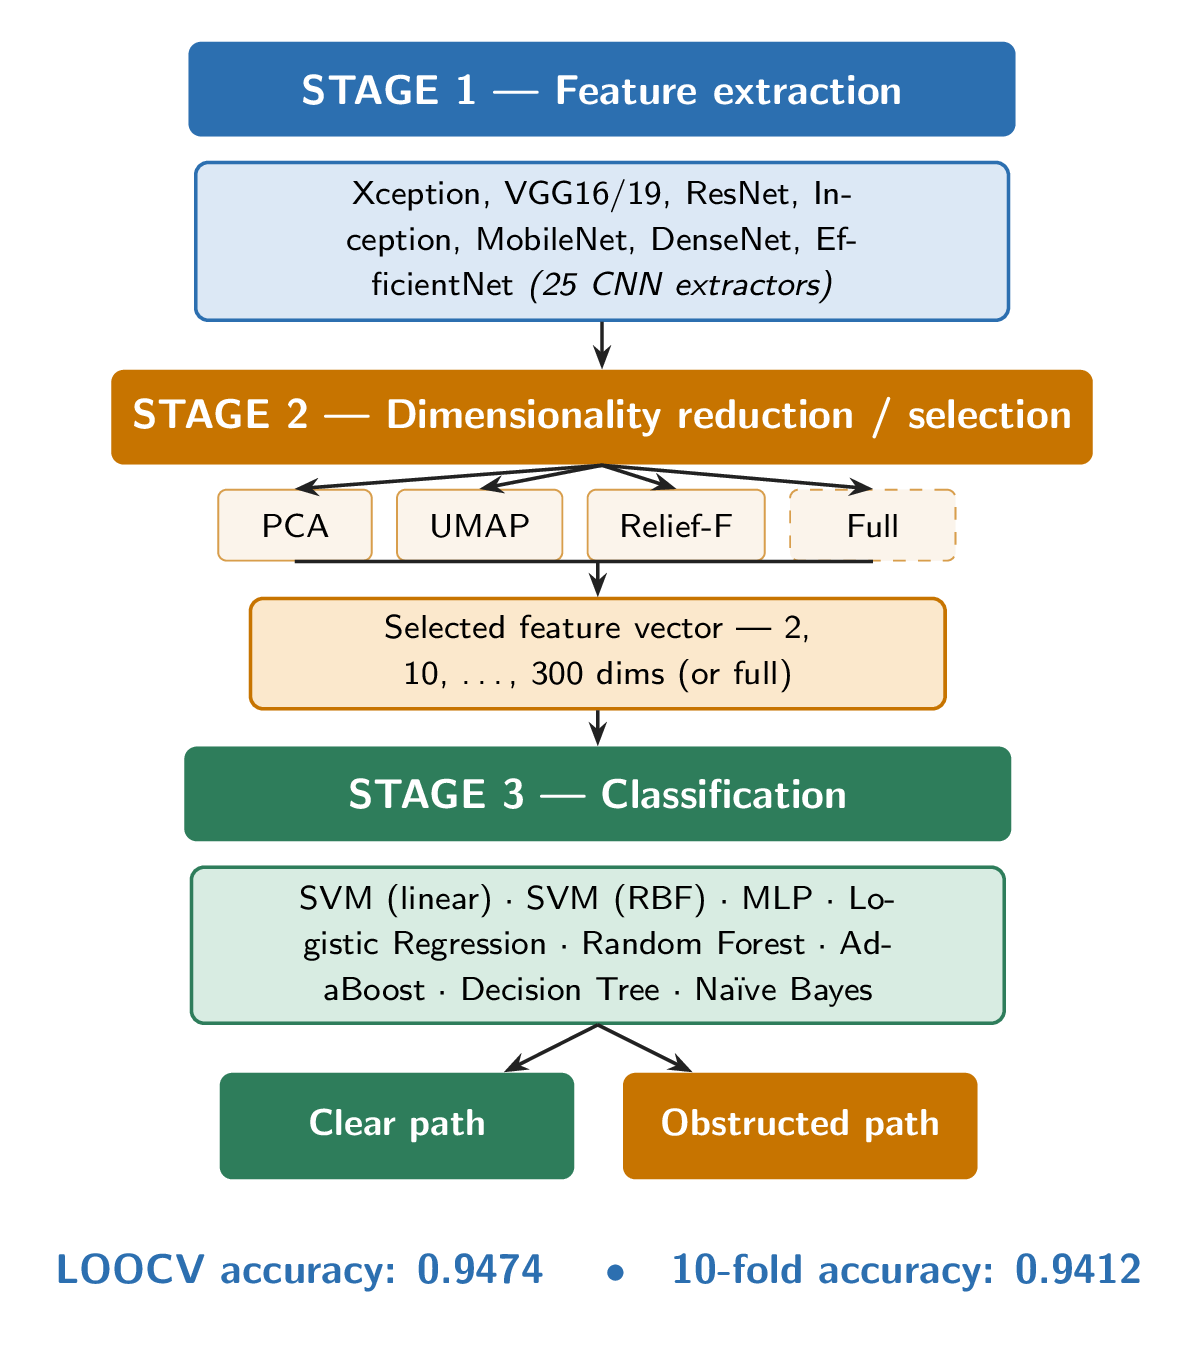
\includegraphics[width=\textwidth]{graphical_abstract.png}
\end{graphicalabstract}

\begin{highlights}
	\item 22 CNN architectures evaluated for obstacle detection in urban navigation.
	\item Features extracted using transfer learning without CNN retraining.
	\item Dimensionality reduction boosted classifier performance and stability.
	\item Best model achieved 95.59\% accuracy with EfficientNetB0 and MobileNet.
	\item The solution is lightweight and suitable for mobile or embedded systems.
\end{highlights}

\begin{keyword}
	Assistive Technology \sep Deep Learning \sep CNN \sep Transfer Learning \sep Dimensionality Reduction \sep Edge Computing \sep Obstacle Detection \sep Visual Impairment
\end{keyword}


%% PACS codes here, in the form: \PACS code \sep code

%% MSC codes here, in the form: \MSC code \sep code
%% or \MSC[2008] code \sep code (2000 is the default)

\end{frontmatter}

%% \linenumbers

%% main text
\section{Introduction}\label{sec:introdution}

Visual impairments, particularly blindness and low vision, represent an escalating challenge for institutions and governments across the globe, as highlighted by the World Health Organization \cite{who2022}. The rising prevalence of eye-related diseases, coupled with a decline in visual acuity, significantly impacts individuals' quality of life and necessitates substantial financial resources for their treatment and rehabilitation \cite{who2022}. Currently, over 2.2 billion individuals suffer from some form of visual impairment, yet access to assistance and services for this demographic remains unequal, according to the United Nations \cite{who2022,bourne2017,onu2019,bourne2020}.

Individuals with visual impairments face numerous challenges in their daily lives, especially in terms of mobility and navigation. Traditionally, this population has relied on canes and guide dogs as their primary means of locomotion \cite{islam2019}. However, advancements in computer vision have led to the development of various navigation systems \cite{islam2019,mandia2023,budrionis2022,kuriakose2021,cardillo2019,bai2019,jiang2019,joe2019,hoang2017,tapu2017,saffoury2016,poggi2016,lakde2015}. It's important to note that many of these systems are limited by the need for expensive, bulky, and/or customized equipment \cite{hoang2017,tapu2017,saffoury2016,poggi2016,poggi2015,rizzo2017}, as well as the requirement for high computational power, rendering them impractical for use on mobile devices. Additionally, some systems necessitate a network connection to a more powerful remote server \cite{jiang2019,lin2017}.

A comprehensive literature review by Budrionis et al. \cite{budrionis2022} revealed that computer vision tools designed for visually impaired individuals operating on smartphones frequently utilize outdated image and video processing techniques. Another literature review by Mandia et al. \cite{mandia2023} found an increasing adoption of deep learning approaches \cite{lecun2015,goodfellow2016,schmidhuber2015}, which has grown in tandem with advancements in computational capabilities. Nonetheless, it is impractical for users to carry high-power computing devices for vision-based assistive solutions. Consequently, there is an increasing need for a deep learning system capable of performing inferences on an edge device, such as a smartphone, without relying on network connectivity or additional accessories.

Breve and Fisher \cite{breve2020} proposed a framework employing Convolutional Neural Networks (CNNs), transfer learning, and semi-supervised learning (SSL) aimed at reducing computational costs and making it feasible for implementation on smartphones without the need for extra hardware. This framework leverages a smartphone's camera to instantly capture images of the user's surroundings and classify them in real time, providing immediate feedback. In this study, a dataset consisting of images from various outdoor and indoor environments under different lighting conditions, floor types, and obstacles was created to facilitate classifier training. The effectiveness of several CNN architectures was assessed by adjusting the pre-trained weights from the ImageNet dataset \cite{russakovsky2015}.

Sanga et al. \cite{sanga2023} developed a prototype based on the framework proposed by Breve and Fisher \cite{breve2020}, consisting of a mobile app that captures video frames from the smartphone's camera, sends them to a server for image classification, and then returns the results to the user. Furthermore, Breve \cite{breve2023} significantly expanded the initial study by incorporating new CNN models, enhancing the cross-validation process, and applying pre-processing functions to improve image preparation. These improvements resulted in enhanced performance in most analyzed cases.

Building on the work of Breve and Fisher \cite{breve2020} and Breve \cite{breve2023}, this paper extends the analysis of using CNNs as feature extractors, exploring various combinations of algorithms for feature extraction, reduction and/or selection, and supervised classifiers. The key contributions are as follows:

1. Exploration of combined approaches involving CNNs, feature reduction and/or selection algorithms, and supervised classifiers.
2. Examination of the full use of CNN-extracted features applied directly to classifiers, without employing dimensionality reduction models.
3. Investigation of the application of dimensionality reduction models to CNN-extracted features prior to classification.
4. Selection of the most effective approaches for the dataset studied.
5. Analysis of classification shortcomings for the selected approaches.

The remainder of the paper is organized as follows: Section 2 presents related work on assistance for visually impaired individuals. Section 3 introduces the dataset used in this study. Section 4 outlines the CNN architectures and algorithms utilized. Section 5 describes the methodology employed. Section 6 discusses the experimental results and analyses, comparing these models' performance on the dataset and exploring deficiencies in the proposed approach. Finally, conclusions are summarized in Section 7. 

\section{Related Works}\label{sec:works}

Several initiatives have been undertaken to incorporate computer vision into assistance for individuals with visual disabilities. Mandia et al. \cite{mandia2023} conducted a comprehensive analysis of current vision-based assistive solutions for visually impaired people.

This analysis primarily focuses on systems utilizing cameras and summarizes the sensors, image processing algorithms, and communication protocols employed. Additionally, the study addresses the use of acoustic output devices, RFID, and GPS, along with cameras. The transition from traditional image processing techniques to the application of deep learning in assisting visually impaired individuals is highlighted. The paper concludes that the literature has not yet fully optimized deep learning models for edge devices.

Budrionis et al. \cite{budrionis2022} provide an overview of recent prototypes of electronic travel aids (ETAs) that utilize smartphones to assist visually impaired individuals with orientation, navigation, and mobility. The authors conduct a systematic review of scientific achievements in this field and compare various smartphone-based ETA prototypes. The meta-analysis identified some attempts to employ cutting-edge computer vision methods based on deep neural networks. The study contrasts these findings with a survey conducted with blind experts to reveal a significant discrepancy between user needs and academic development in the field. The authors conclude that the development of affordable smartphone-based ETAs is crucial for visually impaired people in low-income countries and highlight the need for further research to address the identified gaps.

Islam et al. \cite{islam2019} analyze the development of walking assistants for visually impaired individuals and highlight recent advancements, as well as their advantages and limitations. The authors aim to provide a comprehensive view of the current state of walking assistants and identify areas for future development in sensors, computer vision, and smartphone-based technology.

In turn, Kuriakose et al. \cite{kuriakose2021} propose a scene recognition model based on EfficientNet-Lite for use in a smartphone application that assists in the navigation of blind and visually impaired people. The model is trained and tested using a custom dataset of indoor and outdoor scenes. Additionally, a proof-of-concept prototype of the application was developed on the Android platform.

Bai et al. \cite{bai2019} introduced a wearable assistive device for visually impaired (VI) individuals that aids in navigation and object recognition in both indoor and outdoor environments. The device consists of an RGB-D camera, an inertial measurement unit, a smartphone, and an audio module. It employs a CNN-based object recognition system for perception and navigation. The system provides semantic information about the environment and interacts with the user through audio.

Jiang et al. \cite{jiang2019} proposed a wearable system that utilizes stereo vision. The system leverages binocular vision sensors to capture images and selects the best images based on stereo image quality assessment. The selected images are then sent to the cloud for processing via a convolutional neural network (CNN), and the resulting information is returned to the user to assist in decision-making.

Paul et al. \cite{joe2019} propose a system composed of a camera, GPS, infrared and light sensors connected to a microprocessor (Raspberry Pi) to process and transmit information about the user's environment. The camera captures images, while the microprocessor uses image processing techniques to analyze the images and identify objects and obstacles. The control unit then transmits this information to the user via audio output. The authors did not specify which processing techniques were used, mentioning only the use of the OpenCV library.

Hoang et al. \cite{hoang2017} created a system that uses a Kinect sensor camera mounted on a belt to capture and analyze the surrounding environment. This system identifies obstacles and communicates this information to the user through audio feedback. To process the captured information, it is necessary to carry a laptop in a backpack.

In 2013, Tapu et al. \cite{tapu2013} introduced a real-time obstacle detection and classification system that made use of videos captured by a smartphone's camera. They developed a set of techniques that included tracking, motion estimation, and clustering. Four years later, in 2017, Tapu et al. \cite{tapu2017} presented a more advanced framework based on convolutional neural networks (CNNs) to detect, track, and recognize objects in outdoor environments. However, to run this system, it is necessary to use a laptop computer, which must be carried in a backpack as a processing unit.

Lin et al. \cite{lin2017} introduced a guidance system that makes use of a smartphone. The system incorporates convolutional neural networks (CNNs) for object recognition but requires a desktop server with a GPU and the unified computing device architecture (CUDA) to handle the computationally intensive task of object recognition. Although the system has an offline option, it is limited to recognizing faces and stairs.

Kumar and Meher \cite{kumar2015} introduced an object recognition system that combines the use of CNN (Convolutional Neural Network) and RNN (Recurrent Neural Network). This system is capable of identifying common objects found in indoor environments and their colors, providing auditory feedback to the user. In contrast, Saffoury et al. \cite{saffoury2016} proposed a system that uses a smartphone and a laser pointer. The system employs laser triangulation to establish a collision prevention protocol and provides auditory feedback to the user.

Poggi and Mattoccia \cite{poggi2016} conceived a wearable device composed of a pair of glasses equipped with a custom RGBD sensor and onboard processing performed by an FPGA, a glove with micro-motors for tactile feedback, a portable battery, a bone conduction headset, and a smartphone. This system utilizes deep learning techniques to semantically classify detected obstacles. In a previous work, Poggi et al. \cite{poggi2015} introduced a similar system aimed at recognizing pedestrian crosswalks.

Rizzo et al. \cite{rizzo2017} present a fusion framework that combines signals from a stereo camera and an infrared sensor to detect obstacles using a CNN at multiple scales. They plan to incorporate this framework into a wearable vest.

On the other hand, Islam and Sadi \cite{islam2018} used a CNN to detect potholes in the path and achieved impressive results. However, it is important to note that they used separate datasets for ``path potholes'' and ``non-path potholes'', with the latter including images of roads captured at a wider angle. This raises the possibility that the network learned style differences that are not relevant to the task at hand, simplifying its work.

\section{Dataset}\label{sec:dataset}

The VIA dataset \cite{breve2020} comprises 342 images distributed across two categories: 175 ``clear path'' images and 167 ``obstructed path'' images. The photos were taken using a smartphone camera and resized to 750 × 1000 pixels. The smartphone was held at chest height and tilted at an angle of 30º to 60º to capture several meters of the path ahead, including areas not reached by a standard cane. Despite its modest size, this dataset encompasses a variety of indoor and outdoor environments with different types of flooring, including dry and wet surfaces, natural and artificial lighting conditions, as well as obstacles such as stairs, trees, holes, animals, and traffic cones. Examples of these images can be seen in Fig.~\ref{fig:VIA}.

\begin{figure}
	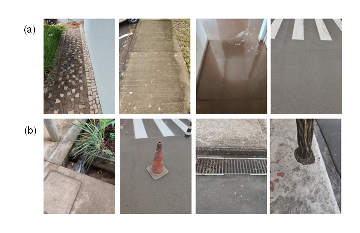
\includegraphics[width=\textwidth]{figVia.eps}
	\caption{Examples from the VIA dataset: (a) “clear path” category; and (b) “path with obstacles” category.} \label{fig:VIA}
\end{figure}


\section{CNN Architectures and Algorithmic Approaches}

This section presents the CNN architectures explored in this study, as well as the feature reduction/selection algorithms and classifiers employed herein.

Table~\ref{tab:CNNArch} displays the 22 evaluated architectures, along with some of their features and literature references. The original CNN architectures were utilized with their existing structures and weights for ImageNet classification \cite{russakovsky2015} through transfer learning, except for the dense classification layers, which were removed.

\begin{table}[h!]
	\caption{CNN Architectures, Input Sizes, and Key Characteristics.}
	\label{tab:CNNArch}
	\centering
	\resizebox{\textwidth}{!}{%
		\begin{tabular}{|l|c|c|c|c|}
			\hline
			\textbf{CNN} & \textbf{Img Res.} & \textbf{Last Conv. (out)} & \textbf{Train. Params} & \textbf{Ref.} \\
			\hline
			DenseNet121 & 224x224 & 7x7x1024 & 8.1M & \cite{huang2017} \\
			DenseNet169 & 224x224 & 7x7x1664 & 14.3M & \cite{huang2017} \\
			DenseNet201 & 224x224 & 7x7x1920 & 20.2M & \cite{huang2017} \\
			EfficientNetB0 & 224x224 & 7x7x1280 & 5.3M & \cite{tan2019} \\
			EfficientNetB1 & 240x240 & 8x8x1280 & 7.9M & \cite{tan2019} \\
			EfficientNetB2 & 260x260 & 9x9x1280 & 9.2M & \cite{tan2019} \\
			EfficientNetB3 & 300x300 & 10x10x1536 & 12.3M & \cite{tan2019} \\
			EfficientNetB4 & 380x380 & 12x12x1792 & 19.5M & \cite{tan2019} \\
			Inception-V3 & 229x229 & 8x8x2048 & 23.9M & \cite{szegedy2016} \\
			Inception-ResNet-V2 & 229x229 & 8x8x1536 & 55.9M & \cite{szegedy2017} \\
			MobileNet & 224x224 & 7x7x1024 & 4.3M & \cite{howard2017} \\
			MobileNetV2 & 224x224 & 7x7x1280 & 3.5M & \cite{sandler2018} \\
			NASNetMobile & 224x224 & 7x7x1056 & 5.3M & \cite{zoph2018} \\
			ResNet50 & 224x224 & 7x7x2048 & 25.6M & \cite{he2016} \\
			ResNet50V2 & 224x224 & 7x7x2048 & 25.6M & \cite{zhang2016} \\
			ResNet101 & 224x224 & 7x7x2048 & 44.7M & \cite{he2016} \\
			ResNet101V2 & 224x224 & 7x7x2048 & 44.7M & \cite{zhang2016} \\
			ResNet152 & 224x224 & 7x7x2048 & 60.4M & \cite{he2016} \\
			ResNet152V2 & 224x224 & 7x7x2048 & 60.4M & \cite{zhang2016} \\
			VGG16 & 224x224 & 7x7x512 & 138.4M & \cite{simonyan2015} \\
			VGG19 & 224x224 & 7x7x512 & 143.7M & \cite{simonyan2015} \\
			Xception & 299x299 & 10x10x2048 & 22.9M & \cite{chollet2017} \\
			\hline
		\end{tabular}%
	}
\end{table}

For dimensionality reduction, the Principal Components Analysis (PCA) \cite{jolliffe2002} and Uniform Manifold Approximation and Projection (UMAP) \cite{mcinnes2021} algorithms were used. Feature selection was also conducted using the Relief-F selection model \cite{kononenko1994}.

For the model classification tests, the following algorithms were employed: Decision Tree \cite{priyanka2020}, Support Vector Machine - SVM with RBF kernel \cite{liu2011}, SVM with linear kernel \cite{lorena2003}, Multilayer Perceptron - MLP \cite{pereira2013}, Logistic Regression \cite{ekstrom2018}, Random Forest \cite{breiman2001}, Adaboost \cite{zhu2009}, and Gaussian Naïve Bayes \cite{gayathri2016}.

\section{Proposed Methodology}

For the comparative evaluation of results, the methodology adopted by Breve and Fisher \cite{breve2020} was defined as the reference model, and different approaches utilizing CNNs, feature reduction/selection algorithms, and classifiers were proposed in the study for classifying the dataset into clear or obstacle-laden paths for visually impaired users.

For the training and testing of reference models, a computer equipped with an AMD Ryzen 9 3900X processor, 64 GB of RAM, Windows 11 operating system, and an NVIDIA GeForce RTX 2060 SUPER graphics card with 8GB of memory and 2,176 CUDA cores was used.

The tests of the proposed approaches were conducted on a notebook with an Intel Core i7-9750H 2.6GHz processor, 32GB of RAM, running a 64-bit POP OS Linux operating system with kernel version 5.17.5. The models were developed in Python language, version 3.9.12, executed on the Anaconda platform where Spyder IDE version 4.1.4 was used.

The tests of the proposed approaches and reference CNNs were carried out using k-fold cross-validation ($k=10$). To verify the test results, the accuracy (acc) was measured at each execution of the classifier. For statistical validation of the results and ranking of the models within each approach, non-parametric tests were used: Kruskal-Wallis and Friedman, through the statistical software IBM SPSS Statistics, version 20.0.0.

\subsection{Baseline CNN}

As a performance benchmark for classifying images into clear paths or paths with obstacles, the training of 22 convolutional network architectures was conducted. The following convolutional neural networks were utilized as presented in Table~\ref{tab:CNNArch}.

Following the approach proposed by Breve and Fisher \cite{breve2020}, from the architectures of each of the convolutional networks, the original pre-trained layers were retained, and new layers were added to the model. These new layers were trained with images from the dataset for the study (fine-tuned), as can be seen in Fig.~\ref{fig:CNNAddLayer}.

\begin{figure}
	\centering
	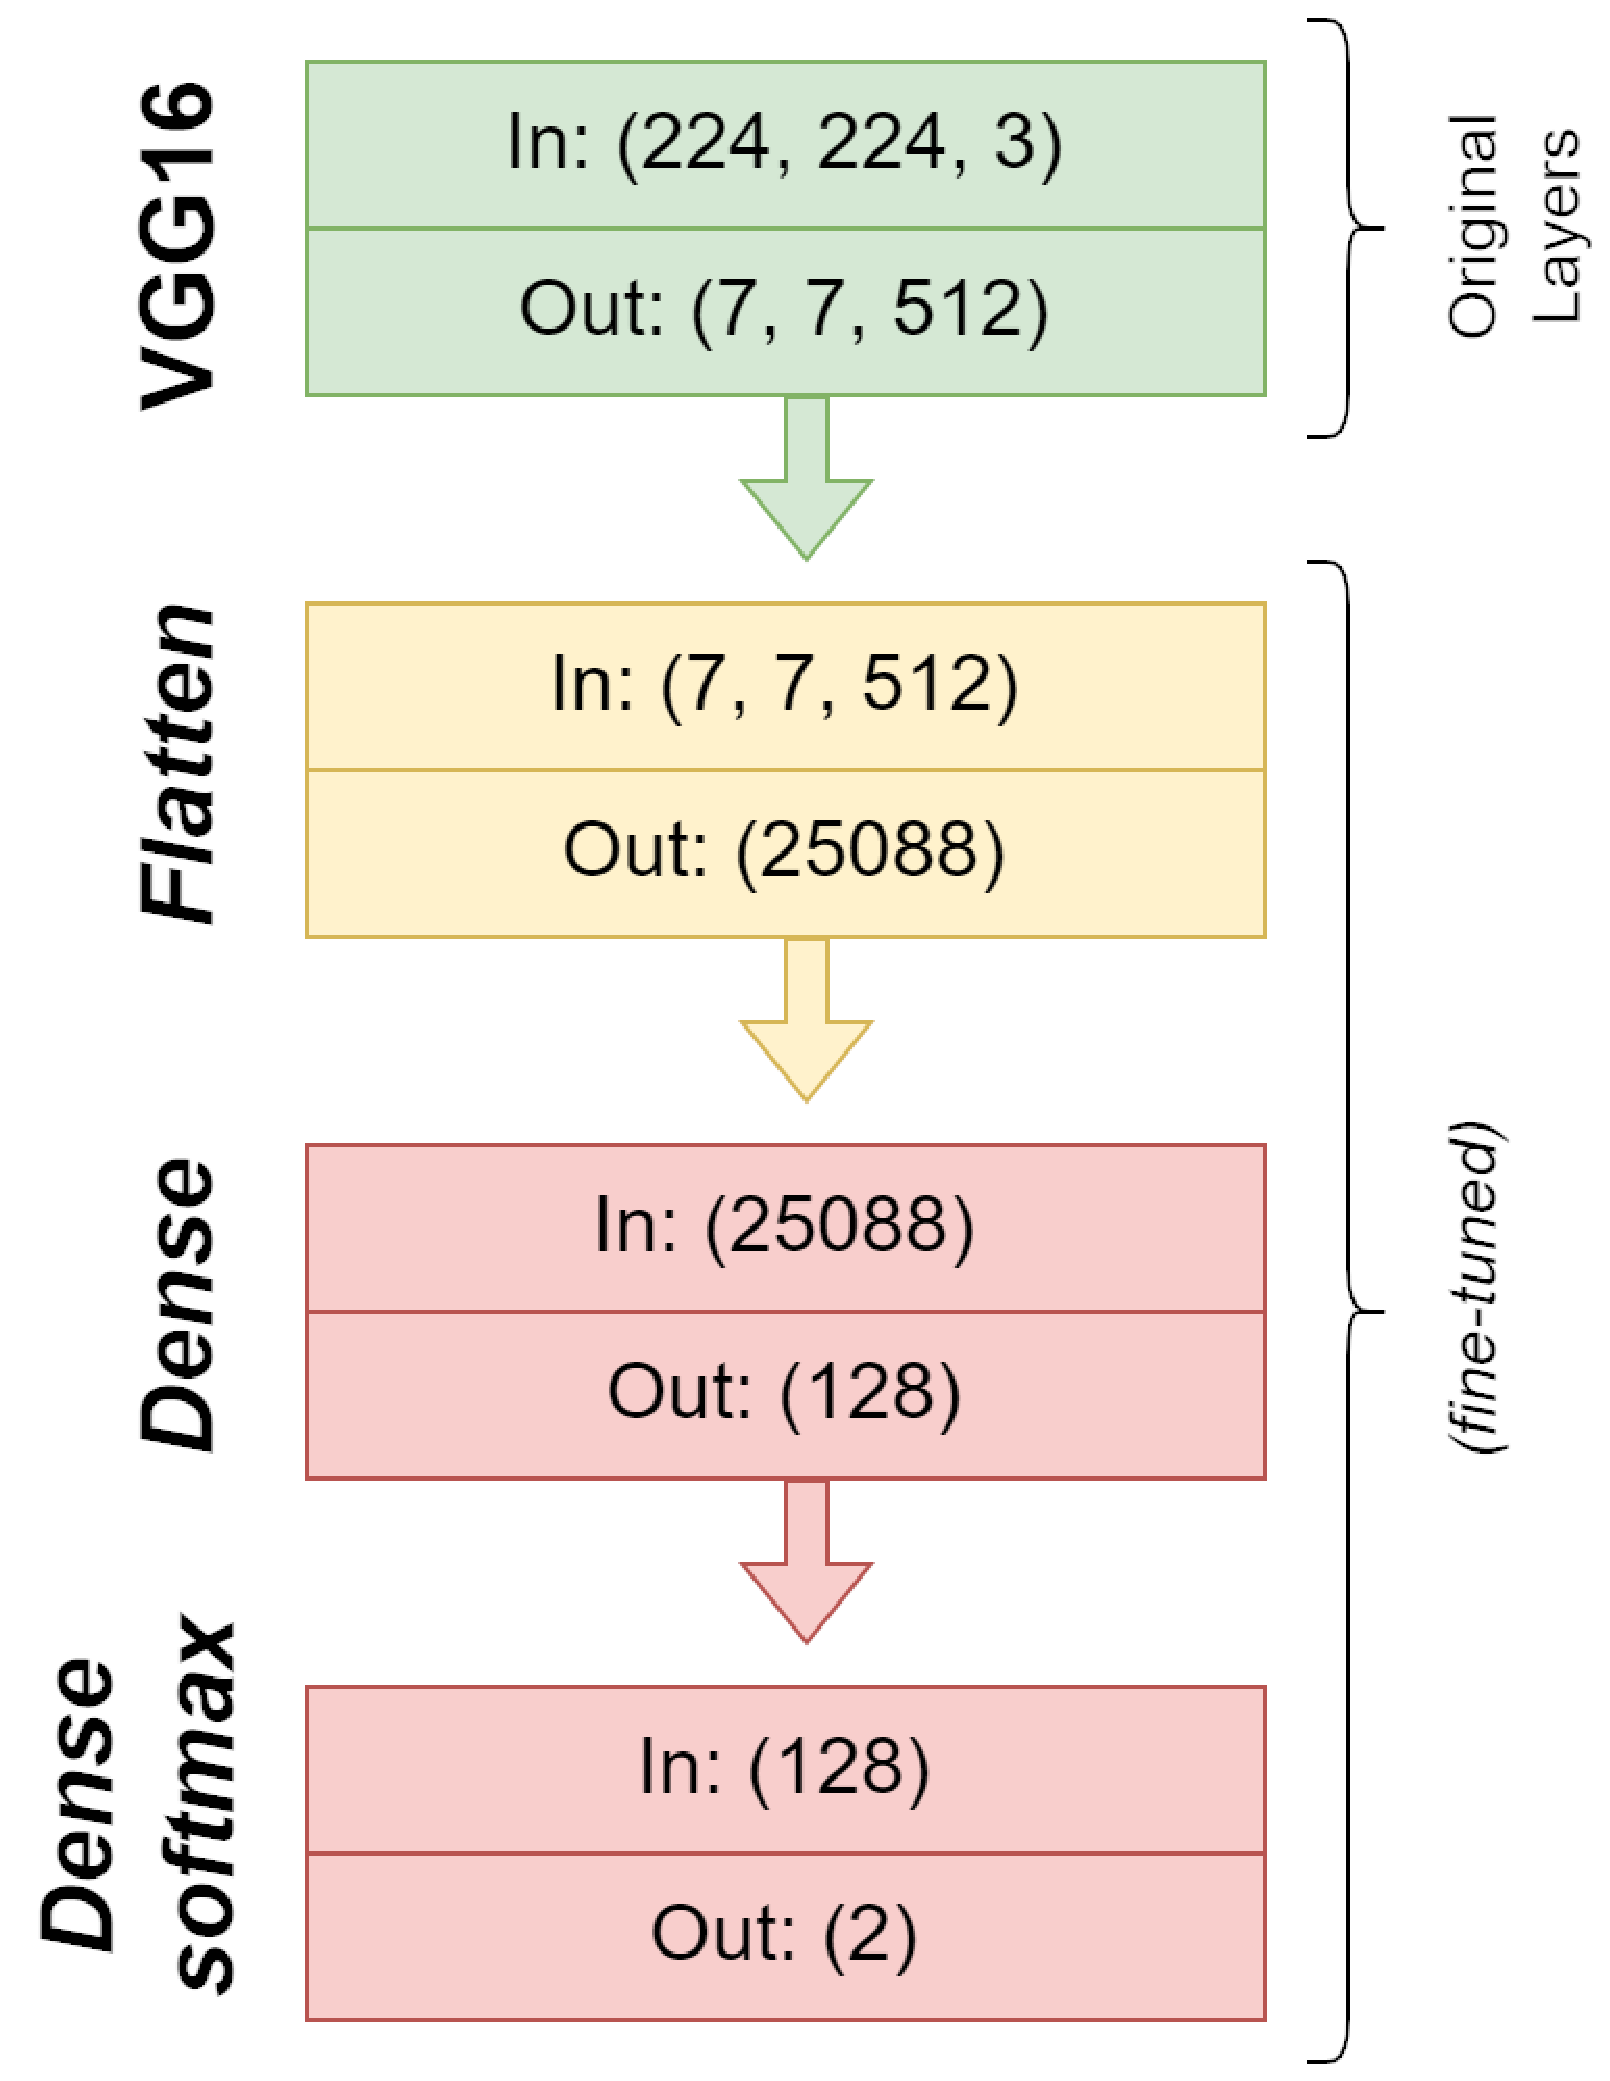
\includegraphics[scale=0.2]{figCNNaddlayer.eps}
	\caption{Layers added to the original CNN Architecture (Example: VGG16).} \label{fig:CNNAddLayer}
\end{figure}

The reference model was evaluated based on the proposed tests to validate the CNN with the best performance for the problem of obstacle identification in the dataset.

\subsection{Approaches Proposed}

The approaches proposed in this study were structured into three stages:

\begin{enumerate}
	\item Feature extraction through CNNs.
	\item Feature reduction or selection.
	\item Classification into clear path or path with obstacles.
\end{enumerate}

For the feature extraction process, the CNNs were not specifically trained for the problem proposed by the work but utilized Transfer Learning with pre-trained parameters from the ImageNet dataset \cite{russakovsky2015}. Thus, information from the last flattened convolutional layer (flatten layer) was used as the feature vector without employing a pooling layer, as illustrated in Fig.~\ref{fig:FeatExtrProcess} with an example from the VGG16 CNN.

\begin{figure}[h!]
	\centering
	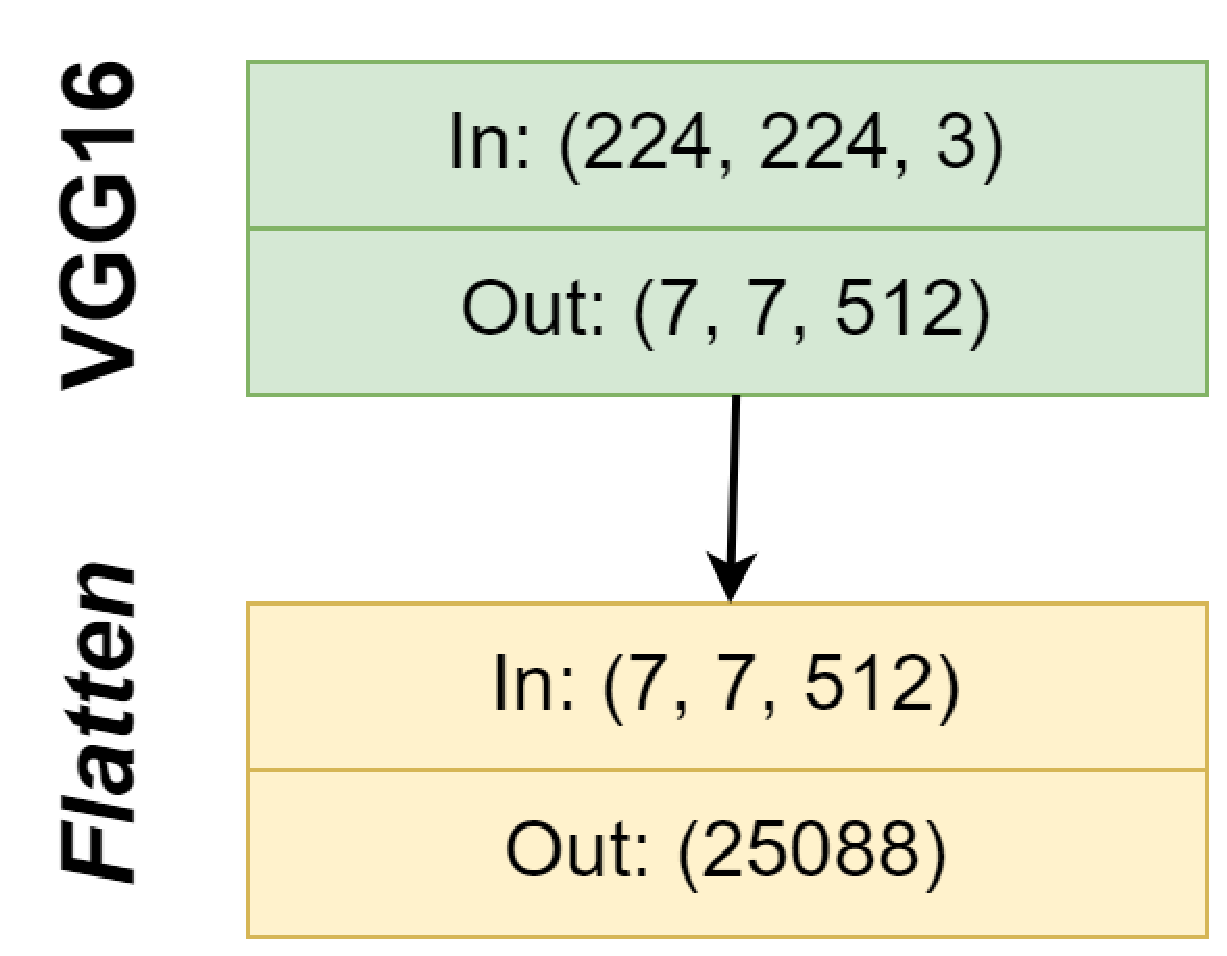
\includegraphics[scale=0.15]{figFeatExtrProcess.eps}
	\caption{Example of the feature extraction process (VGG16).} \label{fig:FeatExtrProcess}
\end{figure}

The second stage of the proposed method involves the use of a model for reduction and/or selection of features or the passing through of all extracted features. The feature reduction algorithms applied were Principal Components Analysis (PCA) \cite{jolliffe2002}, Uniform Manifold Approximation and Projection (UMAP) \cite{mcinnes2021}, and the feature selection algorithm was Relief-F selection model \cite{kononenko1994}. In this phase, when the algorithm was applied, feature vectors of different sizes were generated: 2, 10, 20, 30, 40, 50, 75, 100, 150, 200, 250, and 300 features, reducing the original dimensionality of the output from the convolutional neural network (See: Fig.~\ref{fig:ModelsCombination}).

\begin{figure}[h!]
	\centering
	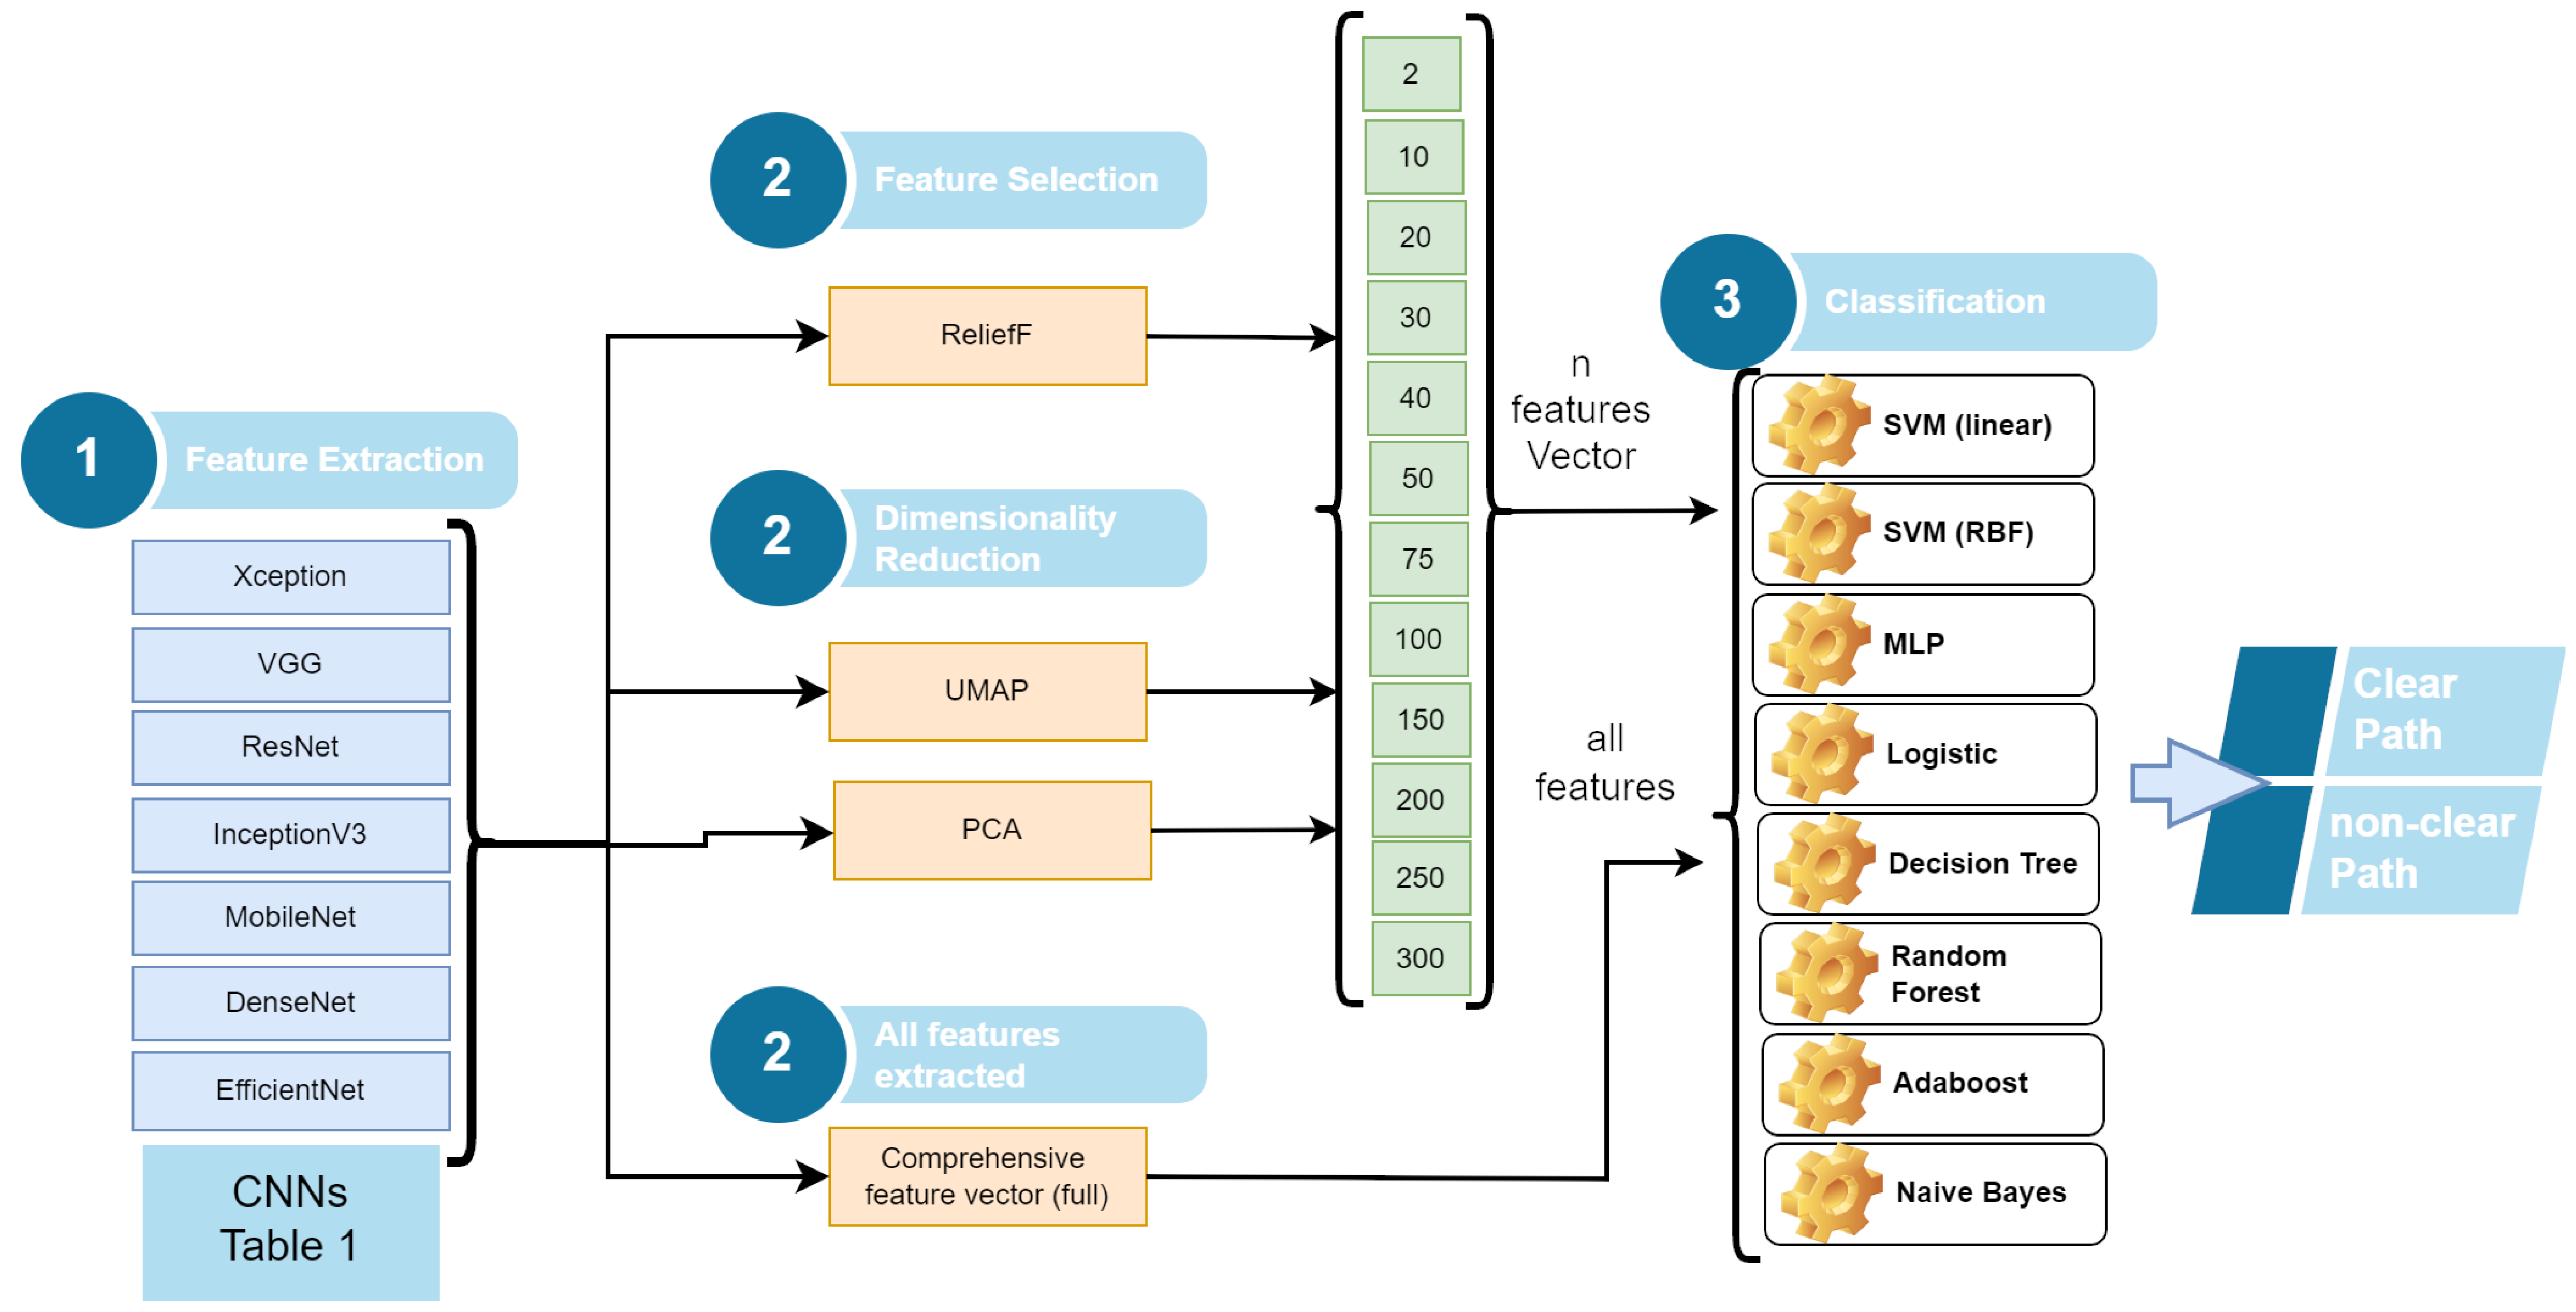
\includegraphics[height=0.35\textheight]{figModelProposed.eps}
	\caption{Combination of possible algorithms at each stage.} \label{fig:ModelsCombination}
\end{figure}

In the third stage, classification is performed using the feature sets presented in stage 2, with the classifiers applied in this phase having been previously introduced.

Fig.~\ref{fig:ModelsCombination} summarizes the resources used for analyzing the proposed model and demonstrates combined approaches of CNN architectures in feature extraction in stage 1 of this model. It can also be concluded that there are many combinations of approaches between stages 1, 2, and 3, thereby structuring four study approaches that we will denote as A, B, C, and D. Tests were initially conducted within each set of the proposed approaches. Within each group of approaches, the model that achieved the highest statistical relevance for the problem was selected.

With the selected models, an analysis was conducted to compare the proposed approaches with the reference model and to produce a ranking among the techniques. Subsequently, a study was also carried out to determine the behavior of the selected models in relation to the classification process for an individual image. For this purpose, leave-one-out cross-validation tests were conducted, as well as an evaluation of the convolutional neural networks through a heatmap analysis.

In approach A, feature extraction was utilized for all the individual CNNs - Fig.~\ref{fig:ApproachA}a and their combinations – Fig.~\ref{fig:ApproachA}b, as demonstrated in Table 2, leveraging the full output of features extracted by the convolutional network without the process of dimensionality reduction, and inputting the data into each of the used classifiers. This approach generated 272 different technique combinations.

In this approach, when combinations of CNNs were used for feature extraction, the output vectors of each of the convolutional networks are concatenated and applied to the classifier (See: Fig.~\ref{fig:ApproachA}b).

\begin{figure}[h!]
	\centering
	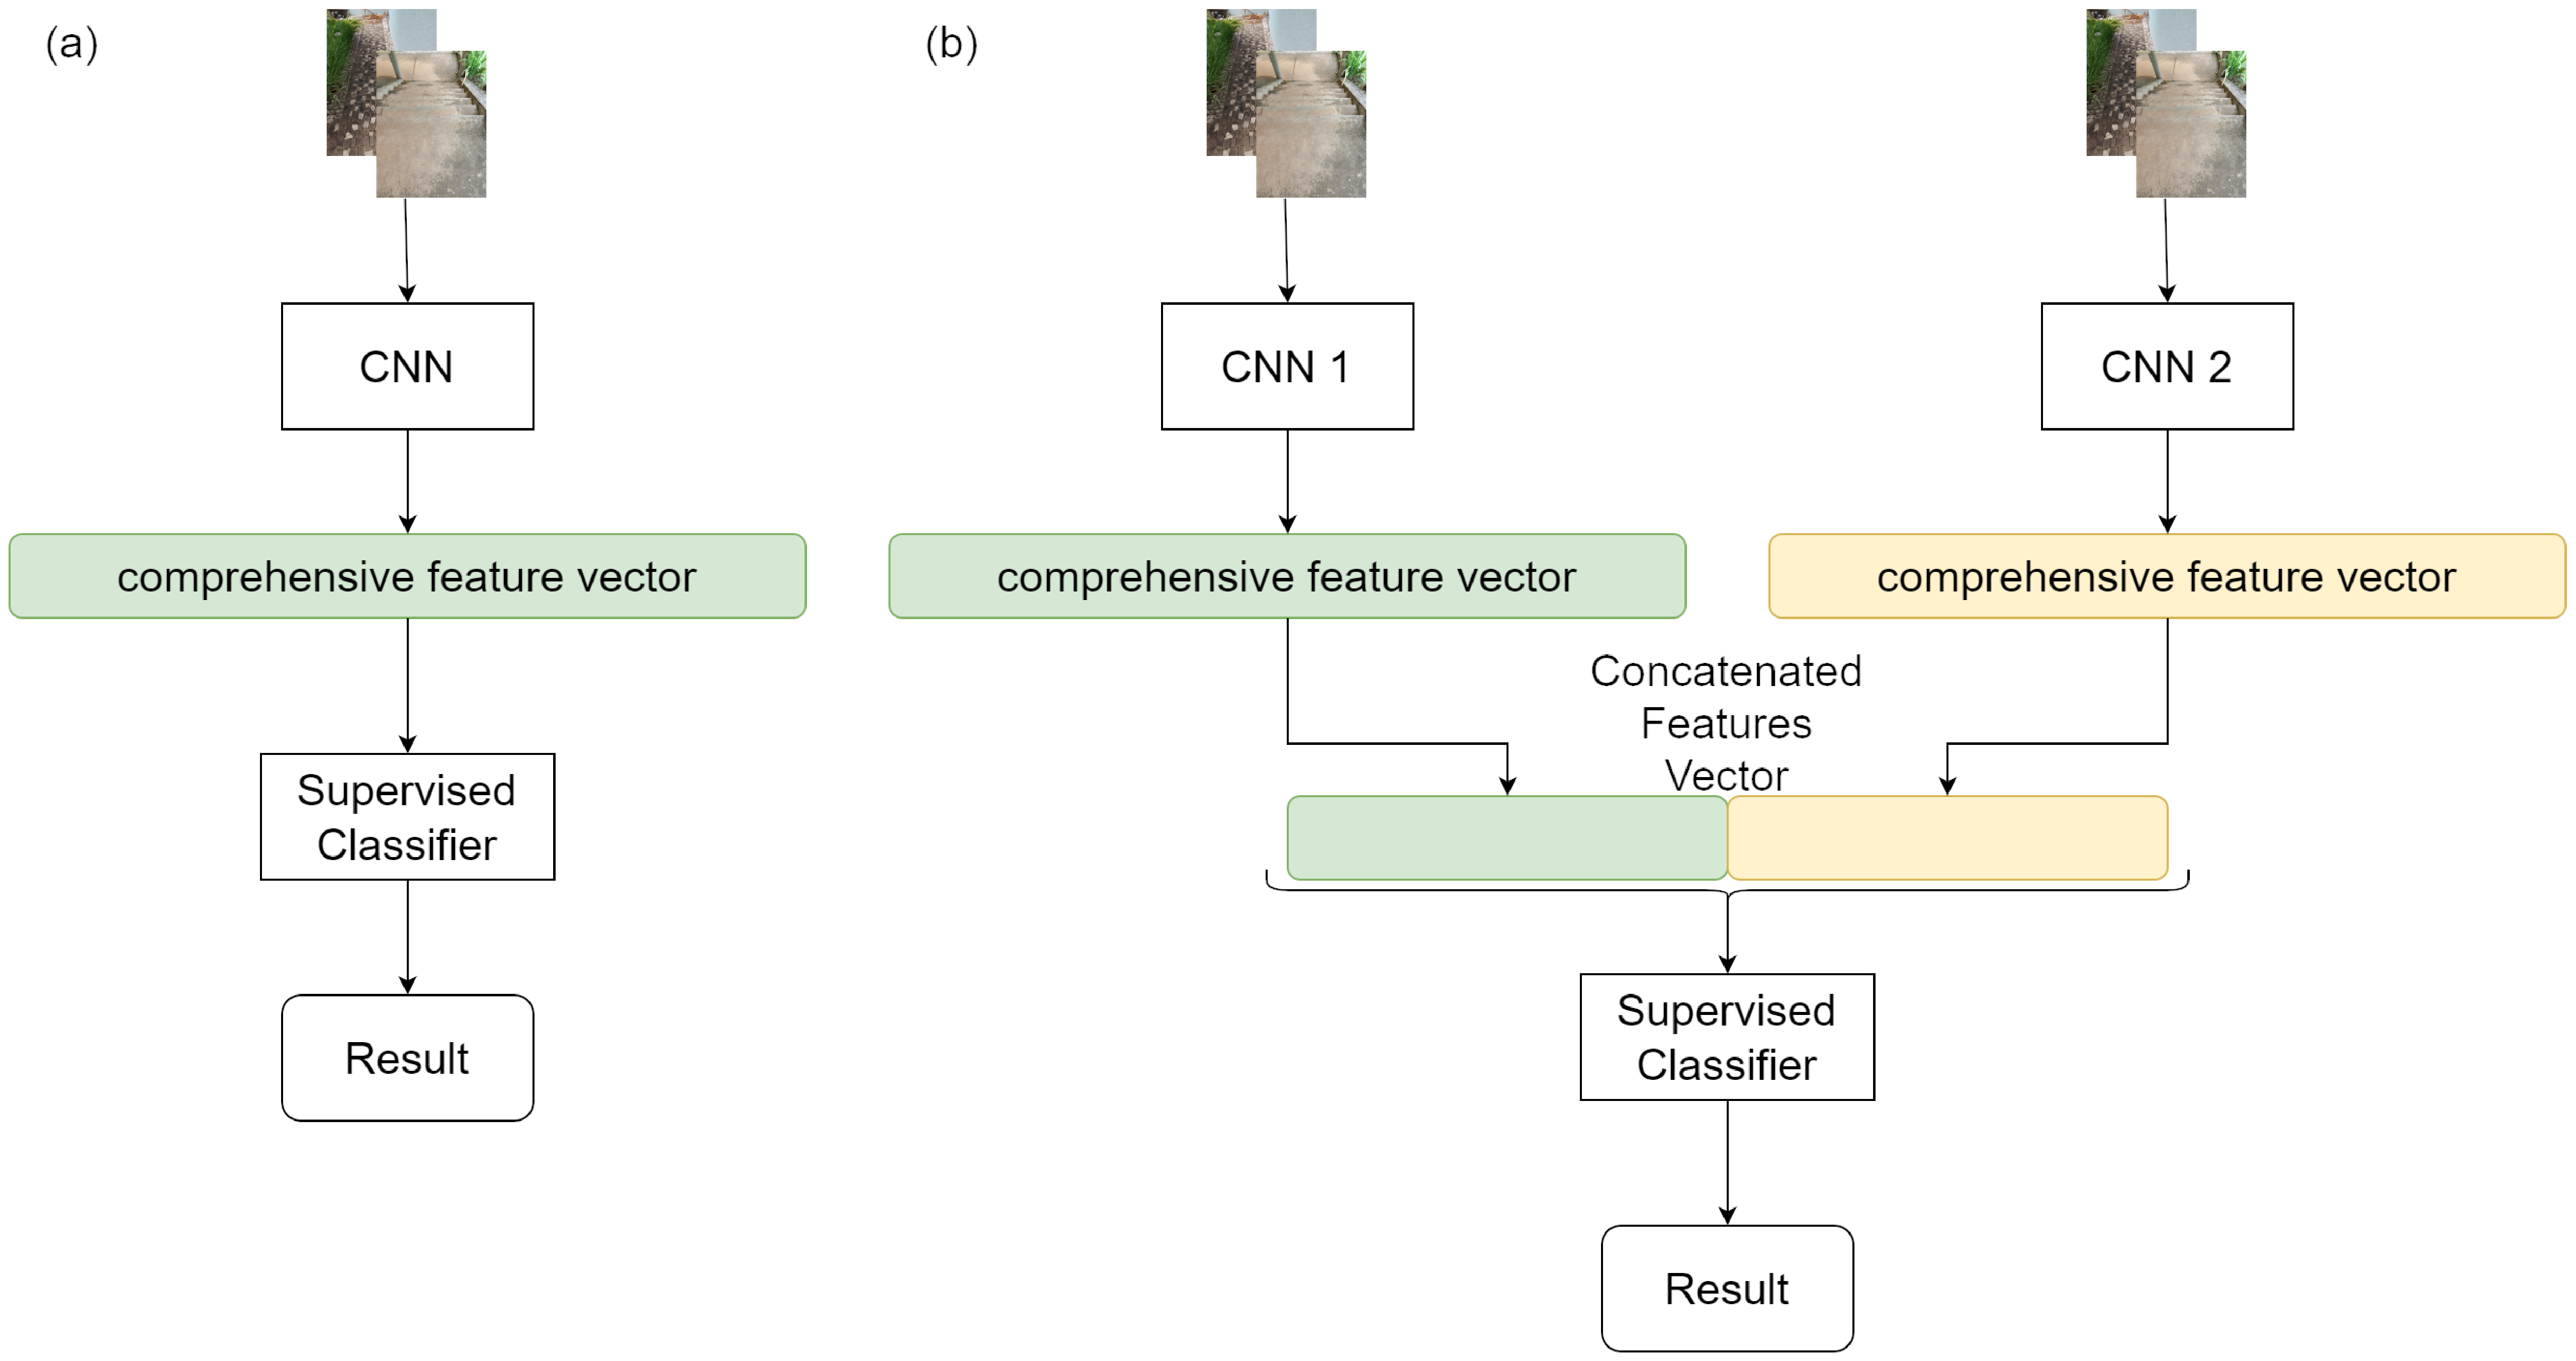
\includegraphics[height=0.3\textheight]{figApproachA.eps}
	\caption{Proposed methodology in Approach A: (a) utilization of the output from only 1 CNN, (b) utilization of the output from 2 CNNs and the concatenation process of the output.} \label{fig:ApproachA}
\end{figure}

In Approach B (Fig.~\ref{fig:ApproachB}), only the individual CNNs were utilized, with the output of features extracted by the convolutional network undergoing a dimensionality reduction process through PCA, UMAP, or Relief-F, where each of the models generated selected feature vectors of sizes 2, 10, 20, 30, 40, 50, 75, 100, 150, 200, 250, and 300. The output vectors generated from the dimensionality reduction process were applied to the 8 classifiers used in this study. This process resulted in 7,200 technique combinations for Approach B.

\begin{figure}[h!]
	\centering
	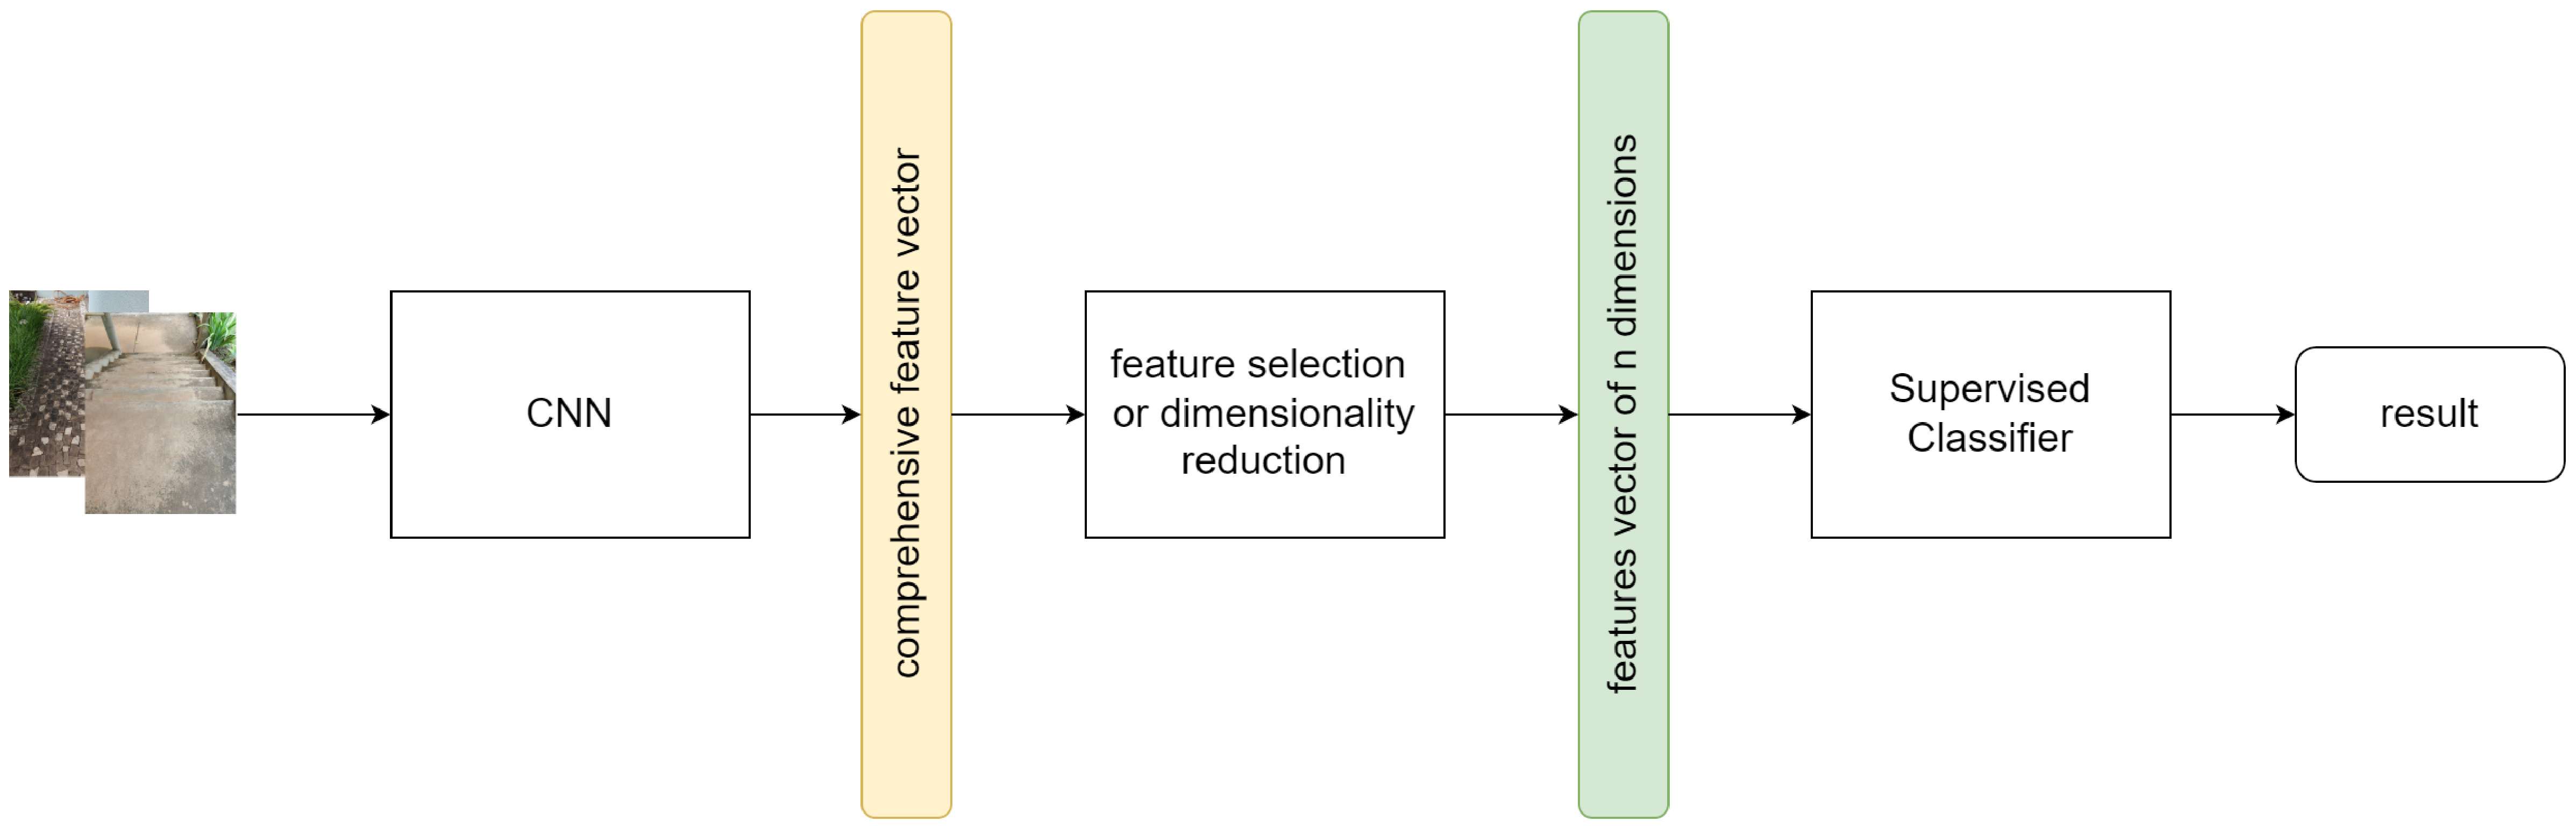
\includegraphics[height=0.2\textheight]{figApproachB.eps}
	\caption{Proposed methodology in Approach B.} \label{fig:ApproachB}
\end{figure}

In Approach C (Fig.~\ref{fig:ApproachC}), combinations of feature vectors extracted from the CNNs were used, as demonstrated in Table 2. 

\begin{figure}[h!]
	\centering
	
\includegraphics[height=0.35\textheight]{figApproachC.eps}
	\caption{Proposed methodology in Approach C.} \label{fig:ApproachC}
\end{figure}

This process involves concatenating the output vectors from each of the applied CNNs into a single vector before subjecting the data to the dimensionality reduction process. The dimensionality reduction utilized the previously worked techniques, PCA, UMAP, and Relief-F, where output vectors of sizes 2, 10, 20, 30, 40, 50, 75, 100, 150, 200, and 300 were generated. Each of these vectors was applied to the 8 classifiers, resulting in a total of 2,592 possible technique combinations for Approach C.

For Approach D (Fig.~\ref{fig:ApproachD}), combinations of feature vectors extracted from the CNNs were also utilized, altering the vector creation process for the classifier. In this approach, each of the utilized CNNs performs feature extraction, and its output vector is subjected to the dimensionality reduction process using one of the proposed techniques, generating the selected feature vector of the desired size (2, 10, 20, 30, 40, 50, 75, 100, 150, 200, or 300). The process occurs individually for each of the CNNs, and only after obtaining the feature vector from each CNN, the feature vector for classification is generated from the concatenation of both. The final vector for classification is subjected to each of the 8 classifiers, resulting in 2,592 possible combinations of the employed techniques.

\begin{figure}[h!]
	\centering
	
\includegraphics[height=0.35\textheight]{figApproachD.eps}
	\caption{Proposed methodology in Approach D.} \label{fig:ApproachD}
\end{figure}

\section{Results}

The tests were conducted using k-fold cross-validation (k=10), and non-parametric Kruskal-Wallis and Friedman tests were performed to determine the best approach for the proposed problem; these tests use the median as a measure of performance.

Given the results presented in the CNN tests, the Null Hypothesis (H0) is that there are no statistically significant differences between their performances, and (H1) such differences exist, making it possible to determine a model suitable for the studied problem.

Upon applying the tests to the reference model, the Kruskal-Wallis test indicated a statistically significant difference among the architectures examined $[X^2(21)=72.822; p<0.0001]$, with the significance level set at $p<0.05$, leading to the rejection of the null hypothesis. Furthermore, to rank the architectures, the Friedman test was utilized $[X^2(21)=75.062; p<0.0001]$. The descriptive outcomes of these performance assessments, which are based on the accuracy achieved and the classification ranking of each studied CNN architecture, are detailed in Table~\ref{tab:Reference_ranking}.

\begin{table}[h!]
	\caption{CNN Architectures and Their Performance Ranking}
	\label{tab:Reference_ranking}
	\centering
	\resizebox{\textwidth}{!}{%
		\begin{tabular}{|l|c|c|c|c|c|}
			\hline
			\textbf{CNN} & \textbf{Rank} & \textbf{Q1 25\%} & \textbf{Q2 50\%} & \textbf{Q3 75\%} & \textbf{IQR} \\
			\hline
			\textbf{DenseNet201} & \textbf{18.25} & \textbf{0.9118} & \textbf{0.9412} & \textbf{0.9416} & \textbf{0.0298} \\
			EfficientNetB0 & 16.65 & 0.8849 & 0.9118 & 0.9412 & 0.0563 \\
			InceptionV3 & 16.65 & 0.9045 & 0.9131 & 0.9486 & 0.0441 \\
			EfficienteNetB3 & 14.55 & 0.8824 & 0.9118 & 0.9210 & 0.0386 \\
			Xception & 14.20 & 0.8750 & 0.8988 & 0.9265 & 0.0515 \\
			EfficientNetB2 & 13.90 & 0.8529 & 0.8971 & 0.9412 & 0.0883 \\
			MobileNet & 13.45 & 0.8677 & 0.8988 & 0.9412 & 0.0735 \\
			EfficientNetB1 & 12.80 & 0.8529 & 0.8971 & 0.9143 & 0.0614 \\
			DenseNet121 & 12.75 & 0.8824 & 0.8841 & 0.9118 & 0.0294 \\
			VGG16 & 12.60 & 0.8456 & 0.8824 & 0.9412 & 0.0957 \\
			DenseNet169 & 12.20 & 0.8561 & 0.8824 & 0.9124 & 0.0564 \\
			ResNet50V2 & 12.15 & 0.8529 & 0.8824 & 0.9210 & 0.0681 \\
			ResNet50 & 11.70 & 0.8456 & 0.8824 & 0.9416 & 0.0961 \\
			VGG19 & 10.80 & 0.8456 & 0.8677 & 0.9192 & 0.0736 \\
			InceptionResnetV2 & 10.30 & 0.8235 & 0.8677 & 0.9210 & 0.0975 \\
			EfficientNetB4 & 10.15 & 0.8456 & 0.8529 & 0.9196 & 0.0740 \\
			ResNet152 & 9.55 & 0.8200 & 0.8677 & 0.9118 & 0.0918 \\
			ResNet152V2 & 8.20 & 0.7941 & 0.8530 & 0.9124 & 0.1183 \\
			ResNet101V2 & 7.35 & 0.8235 & 0.8529 & 0.8824 & 0.0589 \\
			ResNet101 & 7.10 & 0.8235 & 0.8382 & 0.8603 & 0.0368 \\
			MobileNetV2 & 5.00 & 0.7550 & 0.8235 & 0.8603 & 0.1053 \\
			NasNetMobile & 2.80 & 0.5107 & 0.6176 & 0.6912 & 0.1805 \\
			\hline
		\end{tabular}
	}
\end{table}

For the proposed approach A, the tests followed the same standards, wherein the Kruskal-Wallis test made it possible to verify that there is a statistical difference between the architectures studied $[X^2(271)=1,583.052; p<0.0001]$. The significance level of $p<0.05$ determines the rejection of the null hypothesis. In Table~\ref{tab:Approach_A_ranking}, one can observe the descriptive results of the performance tests and the ranking through the Friedman test $[X^2(271)=1,731.191; p<0.0001]$. Due to the large number of combinations of techniques, the twenty highest-ranked techniques were presented.

\begin{table}[h!]
	\caption{Proposed Model – Approach A: Friedman Test ranking and descriptive analysis performance}
	\label{tab:Approach_A_ranking}
	\centering
	\resizebox{\textwidth}{!}{%
		\begin{tabular}{|l|c|c|c|c|c|}
			\hline
			\textbf{} & \textbf{} & \textbf{Q1} & \textbf{Q2} & \textbf{Q3} & \textbf{} \\
			\textbf{Approach A} & \textbf{Rank} & \textbf{25\%} & \textbf{50\%} & \textbf{75\%} & \textbf{IQR} \\
			\hline
			\textbf{EfficientNetB0+} & & & & & \\
			\textbf{MobileNet} & & & & & \\
			\textbf{+LinearSVM} & \textbf{234.75} & \textbf{0.9118} & \textbf{0.9412} & \textbf{0.9706} & \textbf{0.0588} \\
			MobileNet+ResNet50\_ & & & & & \\
			LinearSVM & 230.75 & 0.9273 & 0.9412 & 0.9708 & 0.0435 \\
			EfficienteNetB2\_ & & & & & \\
			LinearSVM & 228.60 & 0.9137 & 0.9412 & 0.9706 & 0.0569 \\
			EfficientNetB0+ & & & & & \\
			MobileNet\_Logistic & 228.25 & 0.9053 & 0.9412 & 0.9706 & 0.0653 \\
			ResNet101+MobileNetV2 & & & & & \\
			\_LinearSVM & 226.65 & 0.9118 & 0.9143 & 0.9706 & 0.0588 \\
			ResNet50\_Logistic & 226.60 & 0.9053 & 0.9421 & 0.9706 & 0.0653 \\
			ResNet50\_LinearSVM & 225.20 & 0.9053 & 0.9274 & 0.9706 & 0.0653 \\
			Xception+ResNet50\_ & & & & & \\
			Logistic & 225.20 & 0.9053 & 0.9274 & 0.9706 & 0.0653 \\
			EfficientNetB3\_ & & & & & \\
			LinearSVM & 224.65 & 0.9118 & 0.9412 & 0.9416 & 0.0298 \\
			MobileNetV2\_LinearSVM & 222.60 & 0.9118 & 0.9421 & 0.9706 & 0.0588 \\
			\hline
		\end{tabular}
	}
\end{table}

The proposed model described in approach B utilized individual CNNs combined with dimensionality reduction models that resulted in output vectors of sizes 2, 10, 20, 30, 40, 50, 75, 100, 150, 200, 250, and 300. These were then applied to 8 studied classifiers, resulting in a considerable number of technique combinations (7200). Thus, the Kruskal-Wallis and Friedman tests were applied to each of the CNNs individually, resulting in 288 technique combinations for each, thereby selecting the best-performing proposal for each CNN.

From this initial selection within approach B, the most relevant technique combinations for this approach were analyzed. The Kruskal-Wallis test yielded a result of $[X^2(24)=49.546; p<0.002]$, confirming statistical differences between the employed techniques. Ranking (Table~\ref{tab:Approach_B_ranking}) was performed using the Friedman test $[X^2(24)=49.546; p<0.0001]$, which identified the best technique within approach B in this study.

\begin{table}[h!]
	\caption{Proposed Model – Approach B: Friedman Test ranking and descriptive analysis performance}
	\label{tab:Approach_B_ranking}
	\centering
	\resizebox{\textwidth}{!}{%
		\begin{tabular}{|l|c|c|c|c|c|}
			\hline
			\textbf{} & \textbf{} & \textbf{Q1} & \textbf{Q2} & \textbf{Q3} & \textbf{} \\
			\textbf{Approach B} & \textbf{Rank} & \textbf{25\%} & \textbf{50\%} & \textbf{75\%} & \textbf{IQR} \\
			\hline
			\textbf{MobileNet\_PCA\_40\_} & & & & & \\
			\textbf{SVM(RBF)} & \textbf{18.25} & \textbf{0.9118} & \textbf{0.9421} & \textbf{0.9706} & \textbf{0.0588} \\
			EfficientNetB1\_PCA\_300\_ &  &  &  &  &  \\
			SVM (linear) & 17.30 & 0.9339 & 0.9412 & 0.9429 & 0.0091 \\
			MobileNetV2\_PCA\_40\_ & & & & & \\
			SVM(RBF) & 17.10 & 0.9118 & 0.9412 & 0.9498 & 0.0380 \\
			EfficientNetB2\_PCA\_250\_ & & & & & \\
			Logistic & 16.20 & 0.8824 & 0.9412 & 0.9706 & 0.0882 \\
			DenseNet121\_PCA\_300\_ & & & & & \\
			Logistic & 15.90 & 0.8824 & 0.9278 & 0.9706 & 0.0882 \\
			EfficientNetB0\_PCA\_300\_ & & & & & \\
			Logistic & 15.70 & 0.9118 & 0.9265 & 0.9416 & 0.0298 \\
			ResNet101V2\_PCA\_30\_ & & & & & \\
			SVM (linear) & 15.50 & 0.8849 & 0.9118 & 0.9706 & 0.0857 \\
			DenseNet201\_PCA\_300\_ & & & & & \\
			Logistic & 15.35 & 0.8824 & 0.9278 & 0.9486 & 0.0662 \\
			EfficientNetB3\_PCA\_250\_ & & & & & \\
			Logistic & 15.30 & 0.9118 & 0.9118 & 0.9429 & 0.0311 \\
			ResNet101\_PCA\_300\_ & & & & & \\
			Logistic & 14.60 & 0.9053 & 0.9118 & 0.9412 & 0.0359 \\
			\hline
		\end{tabular}
	}
\end{table}

As can be seen in Table~\ref{tab:Approach_B_ranking}, the technique involving the CNN MobileNet with dimensionality reduction via PCA, selecting a vector of 40 features, and the SVM classifier with an RBF kernel, achieved the best performance for this approach.

In approach C, combinations of feature vectors extracted from the CNNs were utilized. This process involves concatenating the output vectors from each of the applied CNNs into a single vector before subjecting the data to the dimensionality reduction process. For dimensionality reduction, previously utilized techniques such as PCA, UMAP, and Relief-F were employed, generating selected feature vectors of sizes 2, 10, 20, 30, 40, 50, 75, 100, 150, 200, and 300; each vector was applied to the 8 studied classifiers.

This approach resulted in 2592 possible technique combinations. Accordingly, the Friedman test was conducted to determine the best technique per set of CNNs used in the feature extraction process, and finally, tests were applied to define the best technique for this approach. Separation by CNN sets created analysis groups of 288 different techniques.

From this initial selection within approach C, the most relevant technique combinations for this approach were analyzed, where the Kruskal-Wallis test resulted in $[X^2(8)=22.989; p<0.003]$; it was confirmed that there are statistical differences between the employed techniques. Ranking (Table~\ref{tab:Approach_C_ranking}) was conducted using the Friedman test $[X^2(8)=22.989; p<0.003]$, through which the best technique within approach C was identified.

\begin{table}[h!]
	\caption{Proposed Model – Approach C: Friedman Test ranking and descriptive analysis performance}
	\label{tab:Approach_C_ranking}
	\centering
	\resizebox{\textwidth}{!}{%
		\begin{tabular}{|l|c|c|c|c|c|}
			\hline
			\textbf{} & \textbf{} & \textbf{Q1} & \textbf{Q2} & \textbf{Q3} & \textbf{} \\
			\textbf{Approach C} & \textbf{Rank} & \textbf{25\%} & \textbf{50\%} & \textbf{75\%} & \textbf{IQR} \\
			\hline
			\textbf{MobileNet+ResNet50\_} &  & &  &  &  \\
			\textbf{PCA\_300\_SVM(linear)} & \textbf{7.20} & \textbf{0.9339} & \textbf{0.9559} & \textbf{0.9786} & \textbf{0.0447} \\
			EfficientB0+MobileNet\_ & & & & & \\
			PCA\_300\_SVM(linear) & 6.45 & 0.9412 & 0.9412 & 0.9498 & 0.0086 \\
			ResNet101+DenseNet121\_ & & & & &  \\
			PCA\_300\_Logistic & 5.30 & 0.8849 & 0.9412 & 0.9706 & 0.0857 \\
			MobileNet+ResNet101\_ & & & & &  \\
			PCA\_300\_Logistic & 5.00 & 0.9118 & 0.9412 & 0.9416 & 0.0298 \\
			EfficientNetB1+ &  & &  & & \\
			EfficientNetB5 &  & &  & & \\
			\_PCA\_300\_Logistic & 4.85 & 0.9045 & 0.9278 & 0.9498 & 0.0454 \\
			ResNet101+DenseNet169\_ & & & & & \\
			PCA\_40\_SVM (RBF) & 4.80 & 0.9045 & 0.9143 & 0.9486 & 0.0441 \\
			Xception+ResNet50\_ & & & & &  \\
			PCA\_300\_Logistic & 4.75 & 0.8824 & 0.9265 & 0.9498 & 0.0674 \\
			ResNet101+MobileNetV2\_ &  &  &  &  &  \\
			PCA\_300\_Logistic & 4.30 & 0.9053 & 0.9265 & 0.9416 & 0.0363 \\
			VGG16+VGG19\_ &  &  & &  &  \\
			ReliefF\_300\_SVM (RBF) & 2.35 & 0.8397 & 0.8841 & 0.9412 & 0.1015 \\
			\hline
		\end{tabular}
	}
\end{table}

As can be observed in Table~\ref{tab:Approach_C_ranking}, the technique involving the CNN MobileNet+ ResNet50 with dimensionality reduction via PCA, selecting a vector of 300 features, and the SVM classifier with a linear kernel, achieved the best performance for this approach.

In approach D, the same conditions as approach C apply, with the modification being in the construction of the feature vector where each of the CNNs undergoes a dimensionality reduction process before the merging of the output vectors. This approach resulted in 2592 possible technique combinations. Consequently, the Friedman test was conducted to determine the best technique per set of CNNs used in the feature extraction process, and ultimately, tests were applied to define the best technique for this approach. Separation by CNN groups created analysis groups of 288 different techniques.

From this initial selection within approach D, the most relevant technique combinations for this approach were analyzed, where the Kruskal-Wallis test resulted in $[X^2(8)=7.400; p<0.494]$,  indicating that, as there are no significant statistical differences between the employed techniques. Ranking (Table~\ref{tab:Approach_D_ranking}) was conducted using the Friedman test $[X^2(8)=13.266; p<0.103]$, through which the best technique within approach D was identified.


\begin{table}[h!]
	\caption{Proposed Model – Approach D: Friedman Test ranking and descriptive analysis performance}
	\label{tab:Approach_D_ranking}
	\centering
	\resizebox{\textwidth}{!}{%
		\begin{tabular}{|l|c|c|c|c|c|}
			\hline
			\textbf{} & \textbf{} & \textbf{Q1} & \textbf{Q2} & \textbf{Q3} & \textbf{} \\
			\textbf{Approach D} & \textbf{Rank} & \textbf{25\%} & \textbf{50\%} & \textbf{75\%} & \textbf{IQR} \\
			\hline
			\textbf{MobileNet+ResNet50} &  &  &  &  &  \\
			\textbf{\_PCA\_100\_} & & &  &  & \\
			\textbf{SVM(RBF)} & \textbf{5.95} & \textbf{0.9045} & \textbf{0.9278} & \textbf{0.9708} & \textbf{0.0663} \\
			EfficientNetB0+MobileNet &  &  &  &  &  \\
			\_PCA\_200\_SVM (RBF) & 5.90 & 0.9045 & 0.9412 & 0.9706 & 0.0662 \\
			ResNet101+MobileNetV2 & &  &  &  &  \\
			\_PCA\_75\_SVM (RBF) & 5.65 & 0.8761 & 0.9412 & 0.9708 & 0.0947 \\
			ResNet101+DenseNet121 &  &  &  &  &  \\
			\_PCA\_75\_SVM (RBF) & 5.55 & 0.8981 & 0.9412 & 0.9706 & 0.0725 \\
			ResNet101+DenseNet169 &  &  &  &  &  \\
			\_PCA\_75\_SVM (RBF) & 5.20 & 0.8971 & 0.9412 & 0.9412 & 0.0441 \\
			EfficientNetB1+ &  &  & &  &  \\
			EfficientNetB5 &  &  & &  &  \\
			\_PCA\_300\_Logistic & 5.15 & 0.9045 & 0.9278 & 0.9412 & 0.0368 \\
			MobileNet+ResNet101 &  &  & & &  \\
			\_PCA\_75\_SVM (RBF) & 4.50 & 0.8971 & 0.9412 & 0.9416 & 0.0445 \\
			Xception+ResNet50 & &  &  &  &  \\
			\_PCA\_40\_SVM (RBF) & 4.25 & 0.8849 & 0.9118 & 0.9412 & 0.0563 \\
			VGG16+VGG19\_ReliefF & &  &  &  &  \\
			\_300\_SVM (RBF) & 2.85 & 0.8397 & 0.8971 & 0.9412 & 0.1015 \\
			\hline
		\end{tabular}
	}
\end{table}

As can be observed in Table~\ref{tab:Approach_D_ranking}, the technique involving the CNN MobileNet+ ResNet50 with dimensionality reduction via PCA, selecting a vector of 100 features, and the SVM classifier with an RBF kernel, achieved the best performance for this approach.

In Table~\ref{tab:Approaches_Comparative}, the descriptive performance analysis of the selected approaches from previous tests and the reference model can be seen. The null hypothesis is that the reference model, the CNN DenseNet201 \cite{huang2017}, is the best technique for classifying images as either clear path or with obstacles (H0). If any studied approach performs equally to or better than the reference model (without statistically significant differences), then hypothesis (H1) prevails.

\begin{table}[h!]
	\caption{Descriptive Performance Analysis of the Selected Techniques in the studied approaches and the reference model.}
	\label{tab:Approaches_Comparative}
	\centering
	\resizebox{\textwidth}{!}{%
		\begin{tabular}{|l|l|c|c|c|c|}
			\hline
			\textbf{Proposed} & \textbf{} & \textbf{Q1} & \textbf{Q2} & \textbf{Q3} & \textbf{} \\
			\textbf{Model} & \textbf{Appr.} & \textbf{25\%} & \textbf{50\%} & \textbf{75\%} & \textbf{IQR} \\
			\hline
			DenseNet201 & Ref. & 0.9118 & 0.9412 & 0.9416 & 0.0298 \\
			EfficientNetB0+MobileNet & A & 0.9118 & 0.9412 & 0.9706 & 0.0588 \\
			MobileNet PCA\_40\_ &  &  &  &  &  \\
			SVM (RBF) & B & 0.9118 & 0.9421 & 0.9706 & 0.0588 \\
			MobileNet+ResNet50 &  &  &  &  &  \\
			PCA\_300\_SVM (linear) & C & 0.9339 & 0.9559 & 0.9786 & 0.0447 \\
			MobileNet+ResNet50 &  &  &  &  &  \\
			PCA\_100\_SVM (RBF) & D & 0.9045 & 0.9278 & 0.9708 & 0.0663 \\
			\hline
		\end{tabular}
	}
\end{table}

Once the most relevant technique combinations for each of the proposed approaches and the reference model were defined, the Kruskal-Wallis test was applied, yielding a result of $[X^2(4)=1.609; p=0.807]$. This maintains H1 as a valid hypothesis, indicating that, as there are no significant differences between the methods, the studied approaches achieved the objective of classifying images without the need for training a convolutional neural network.

The Friedman test was applied to the approaches and the reference model to rank the best combinations of techniques. The test results were $[X^2(4)=3.477; p=0.481]$, meaning there are no statistically significant differences between the studied approaches and the reference model, rejecting the null hypothesis (H0). In Table~\ref{tab:Approaches_friedman_ranking}, the ranked techniques can be observed from the highest to the lowest score, as a result of the Friedman test.

\begin{table}[h!]
	\centering
	\caption{Friedman Test for the Selected Approaches and the Reference Model}
	\label{tab:Approaches_friedman_ranking}
	\resizebox{\textwidth}{!}{%
		\begin{tabular}{|l|c|}
			\hline
			\textbf{Proposed} & \textbf{Friedman} \\
			\textbf{Model} & \textbf{(Rank)} \\
			\hline
			\textbf{Approach C:} &  \\
			\textbf{MobileNet+ResNet50 PCA\_300\_SVM (linear)} & \textbf{3.70} \\
			Approach A: EfficientNetB0+MobileNet SVM (linear) & 2.95 \\
			Reference Model: DenseNet201 & 2.90 \\
			Approach B: MobileNet PCA\_40\_SVM (RBF) & 2.80 \\
			Approach D: MobileNet+ResNet50 PCA\_100\_SVM (RBF) & 2.65 \\
			\hline
		\end{tabular}
	}
\end{table}

In the ranking, it is observed that approach C, utilizing the CNN MobileNet and CNN ResNet50 with the PCA technique for reducing the dimensionality of the extracted data to 300 features, and the SVM classifier with a linear kernel, was ranked highest. 

Despite the lack of statistical significance, the reference model imposes a much higher computational burden resources for CNN training, whereas the proposed approaches do not involve training a convolutional neural network, only the classifier.

Given the small size of the dataset, a leave-one-out cross-validation (LOOCV) test was chosen for each of the selected approaches, where each sample is used as the test set and the remaining $(N-1)$ samples are used as the training set.

In the test for each image, features were extracted from the training group and the test image, along with the processes of dimensionality reduction and classifier training. In Table~\ref{tab:Kfold_LOOCV_accuracy_comparison}, the performance of the approaches in the conducted test can be observed.

\begin{table}[h!]
	\centering
	\caption{Accuracy in the Leave-One-Out Cross-Validation Test}
	\label{tab:Kfold_LOOCV_accuracy_comparison}
	\resizebox{\textwidth}{!}{%
		\begin{tabular}{|p{8.5cm}|c|c|}
			\hline
			\textbf{Proposed} & \textbf{LOOCV} & \textbf{10-fold} \\
			\textbf{Model} & \textbf{Accuracy} & \textbf{Accuracy} \\
			\hline
			\textbf{Approach A: EfficientNetB0+MobileNet SVM (linear)} & \textbf{0.9474} & \textbf{0.9412} \\
			Approach B: MobileNet PCA\_40\_SVM (RBF) & 0.8713 & 0.9421 \\
			Approach C: MobileNet+ResNet50 PCA\_300\_SVM (linear) & 0.8421 & 0.9559 \\
			Approach D: MobileNet+ResNet50 PCA\_100\_SVM (RBF) & 0.8509 & 0.9278 \\
			\hline
		\end{tabular}
	}
\end{table}

In Table~\ref{tab:Kfold_LOOCV_accuracy_comparison}, it is observed that approach A was the only one to achieve similar performance in both tests conducted, while approaches B, C, and D showed a reduction in accuracy when the images were tested individually.

From this test, images that most frequently exhibited prediction errors with the tested approaches were tabulated. Out of the 342 images used in the tests, 100 images had at least one prediction error in some of the approaches, equating to 29.23\%. Of these 100 images, in 6 images all 4 approaches made a wrong prediction, in 12 images at least 3 approaches incurred an error, in 25 images at least 2 approaches made a wrong prediction, and in 57 images at least one approach erred in classification. Of the 100 images with erroneous classification, 51 represented paths with obstacles and 49 paths without obstacles.

Of the 6 images with errors in all approaches, 2 are of paths without obstacles as can be seen in Fig.~\ref{fig:Heatmap_clean_4}. The demonstrated images are overlaid with a heatmap produced by a technique proposed by Selvaraju et al \cite{selvaraju2020}, where a visual explanation is provided through the mapping of CNN activation.

\begin{figure}[h!]
	\centering
	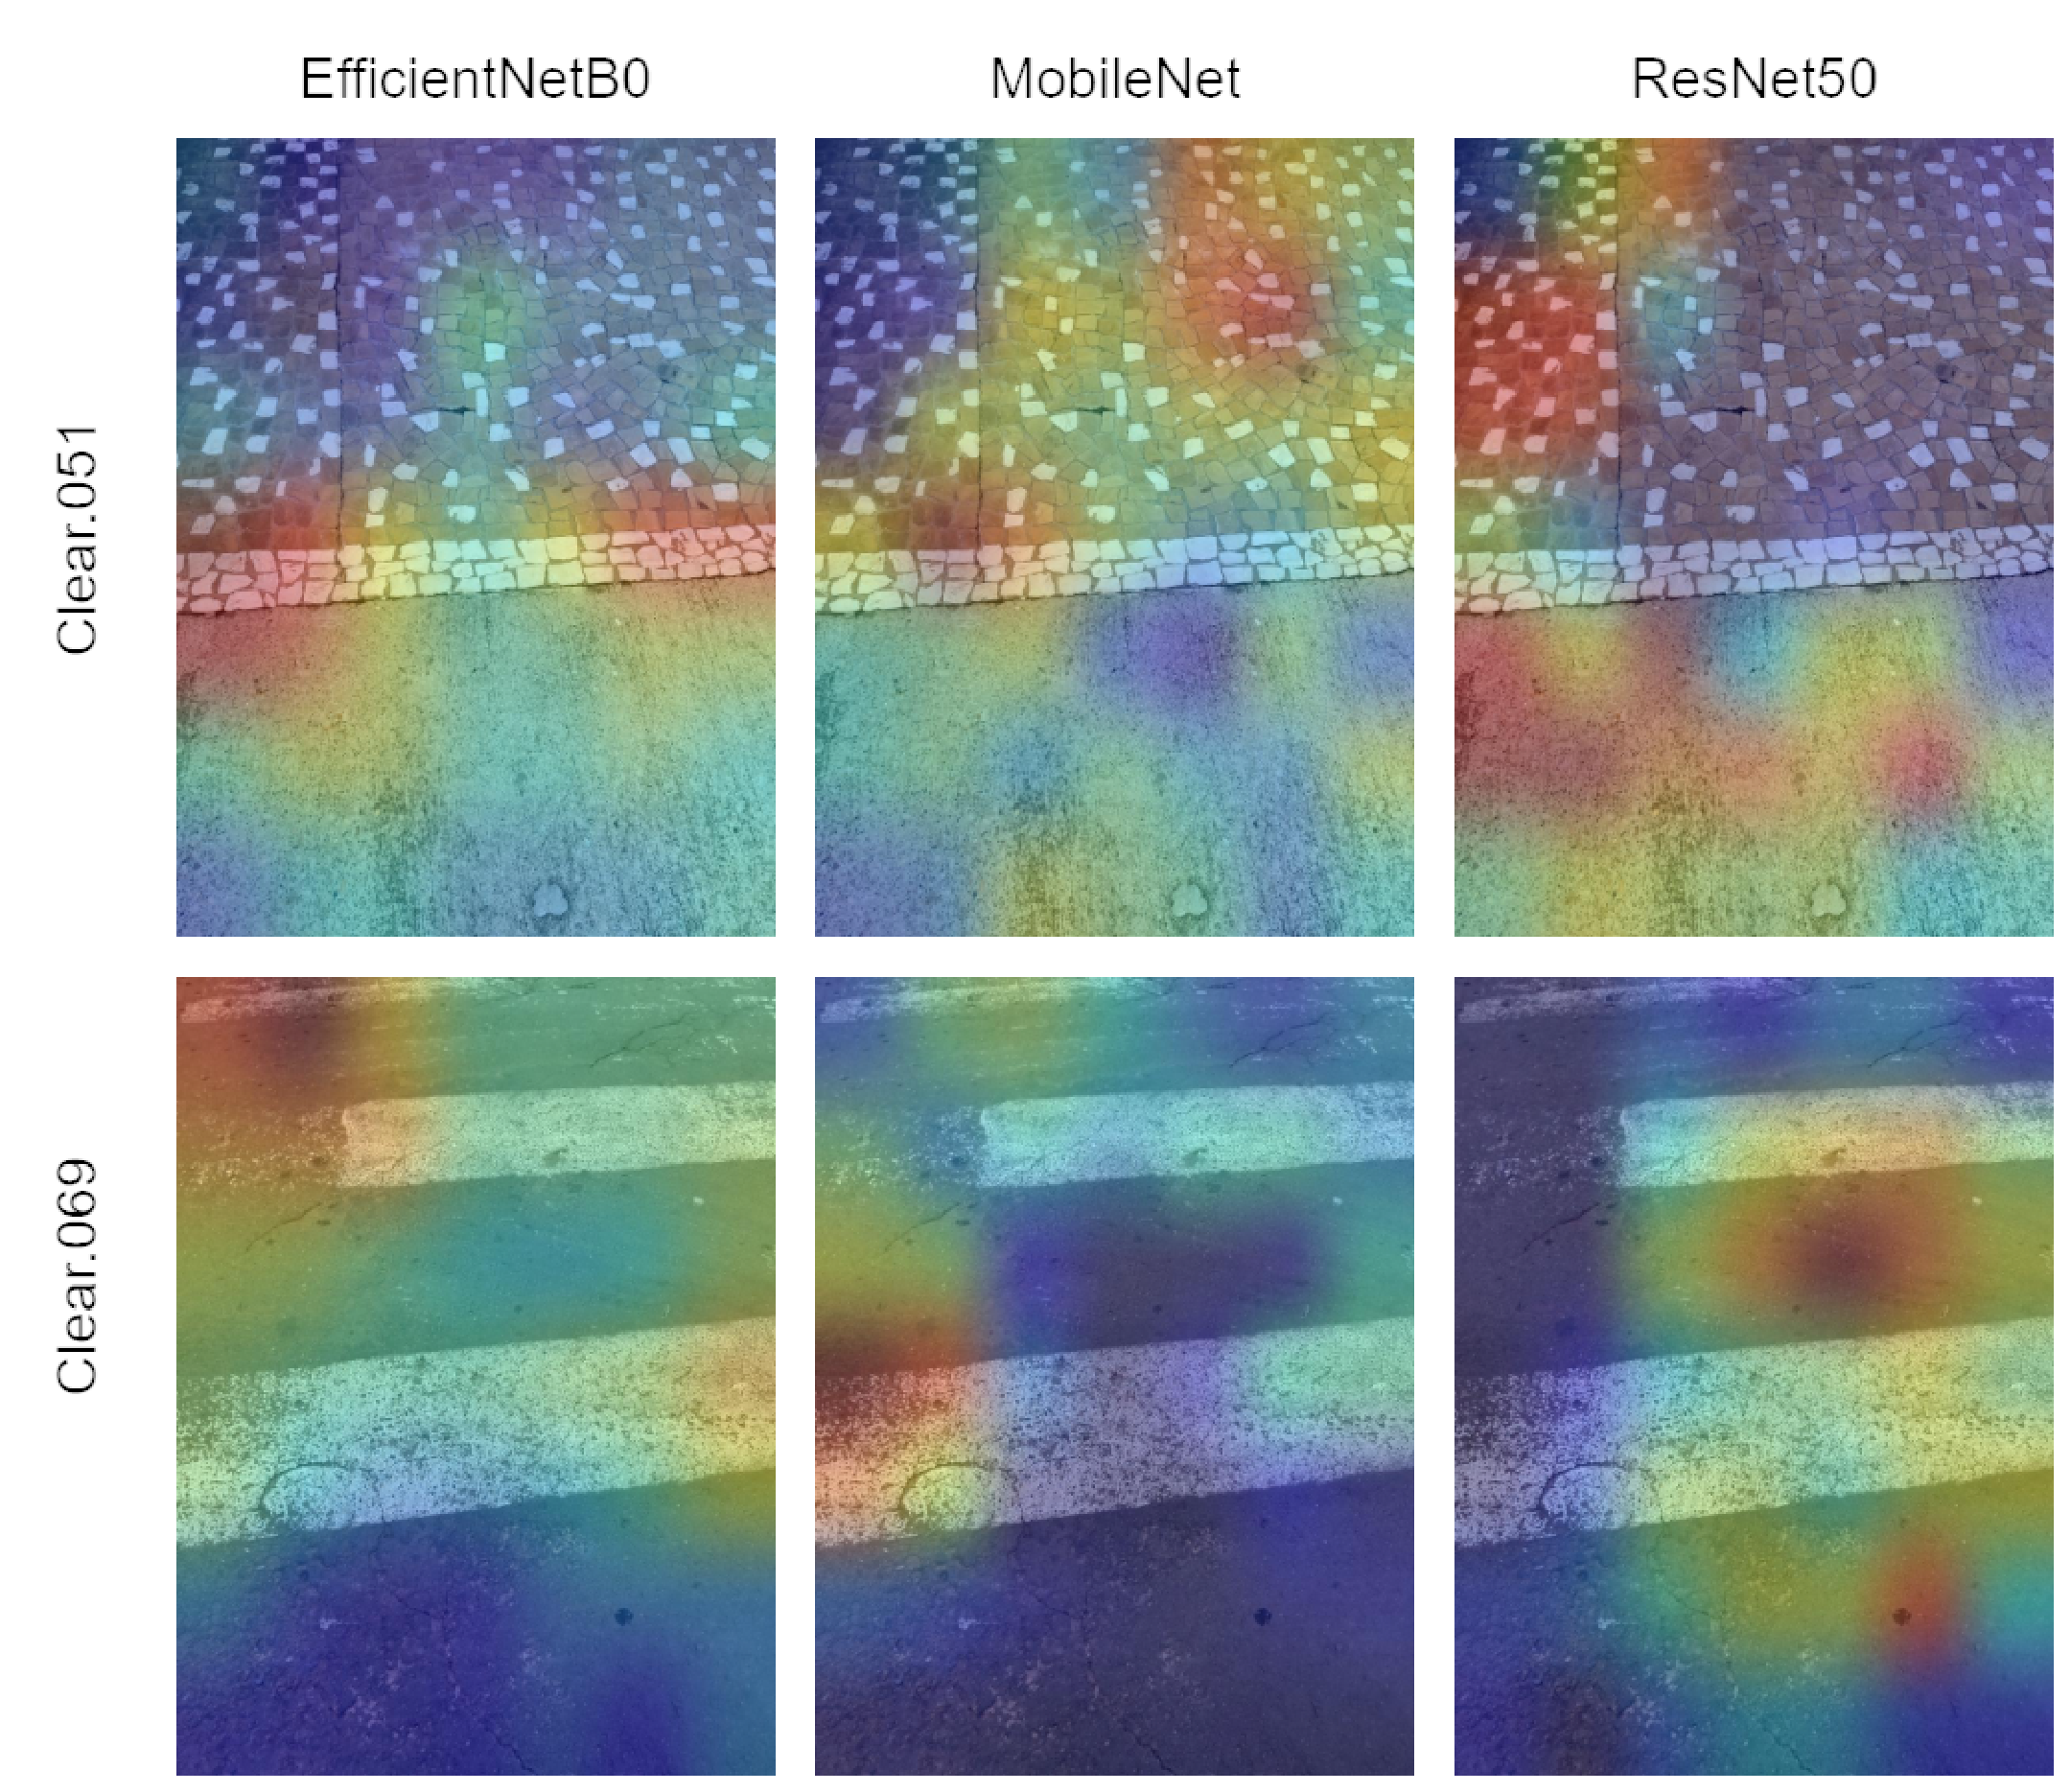
\includegraphics[height=0.5\textheight]{figHeatmap_clean_4.eps}
	\caption{Heatmap of Misclassified Obstructed Paths (All Approaches).} \label{fig:Heatmap_clean_4}
\end{figure}

Among the 6 images with errors in all approaches, 4 were of paths with obstacles, as can be seen in Fig.~\ref{fig:Heatmap_obstacle_4}.

\begin{figure}[h!]
	\centering
	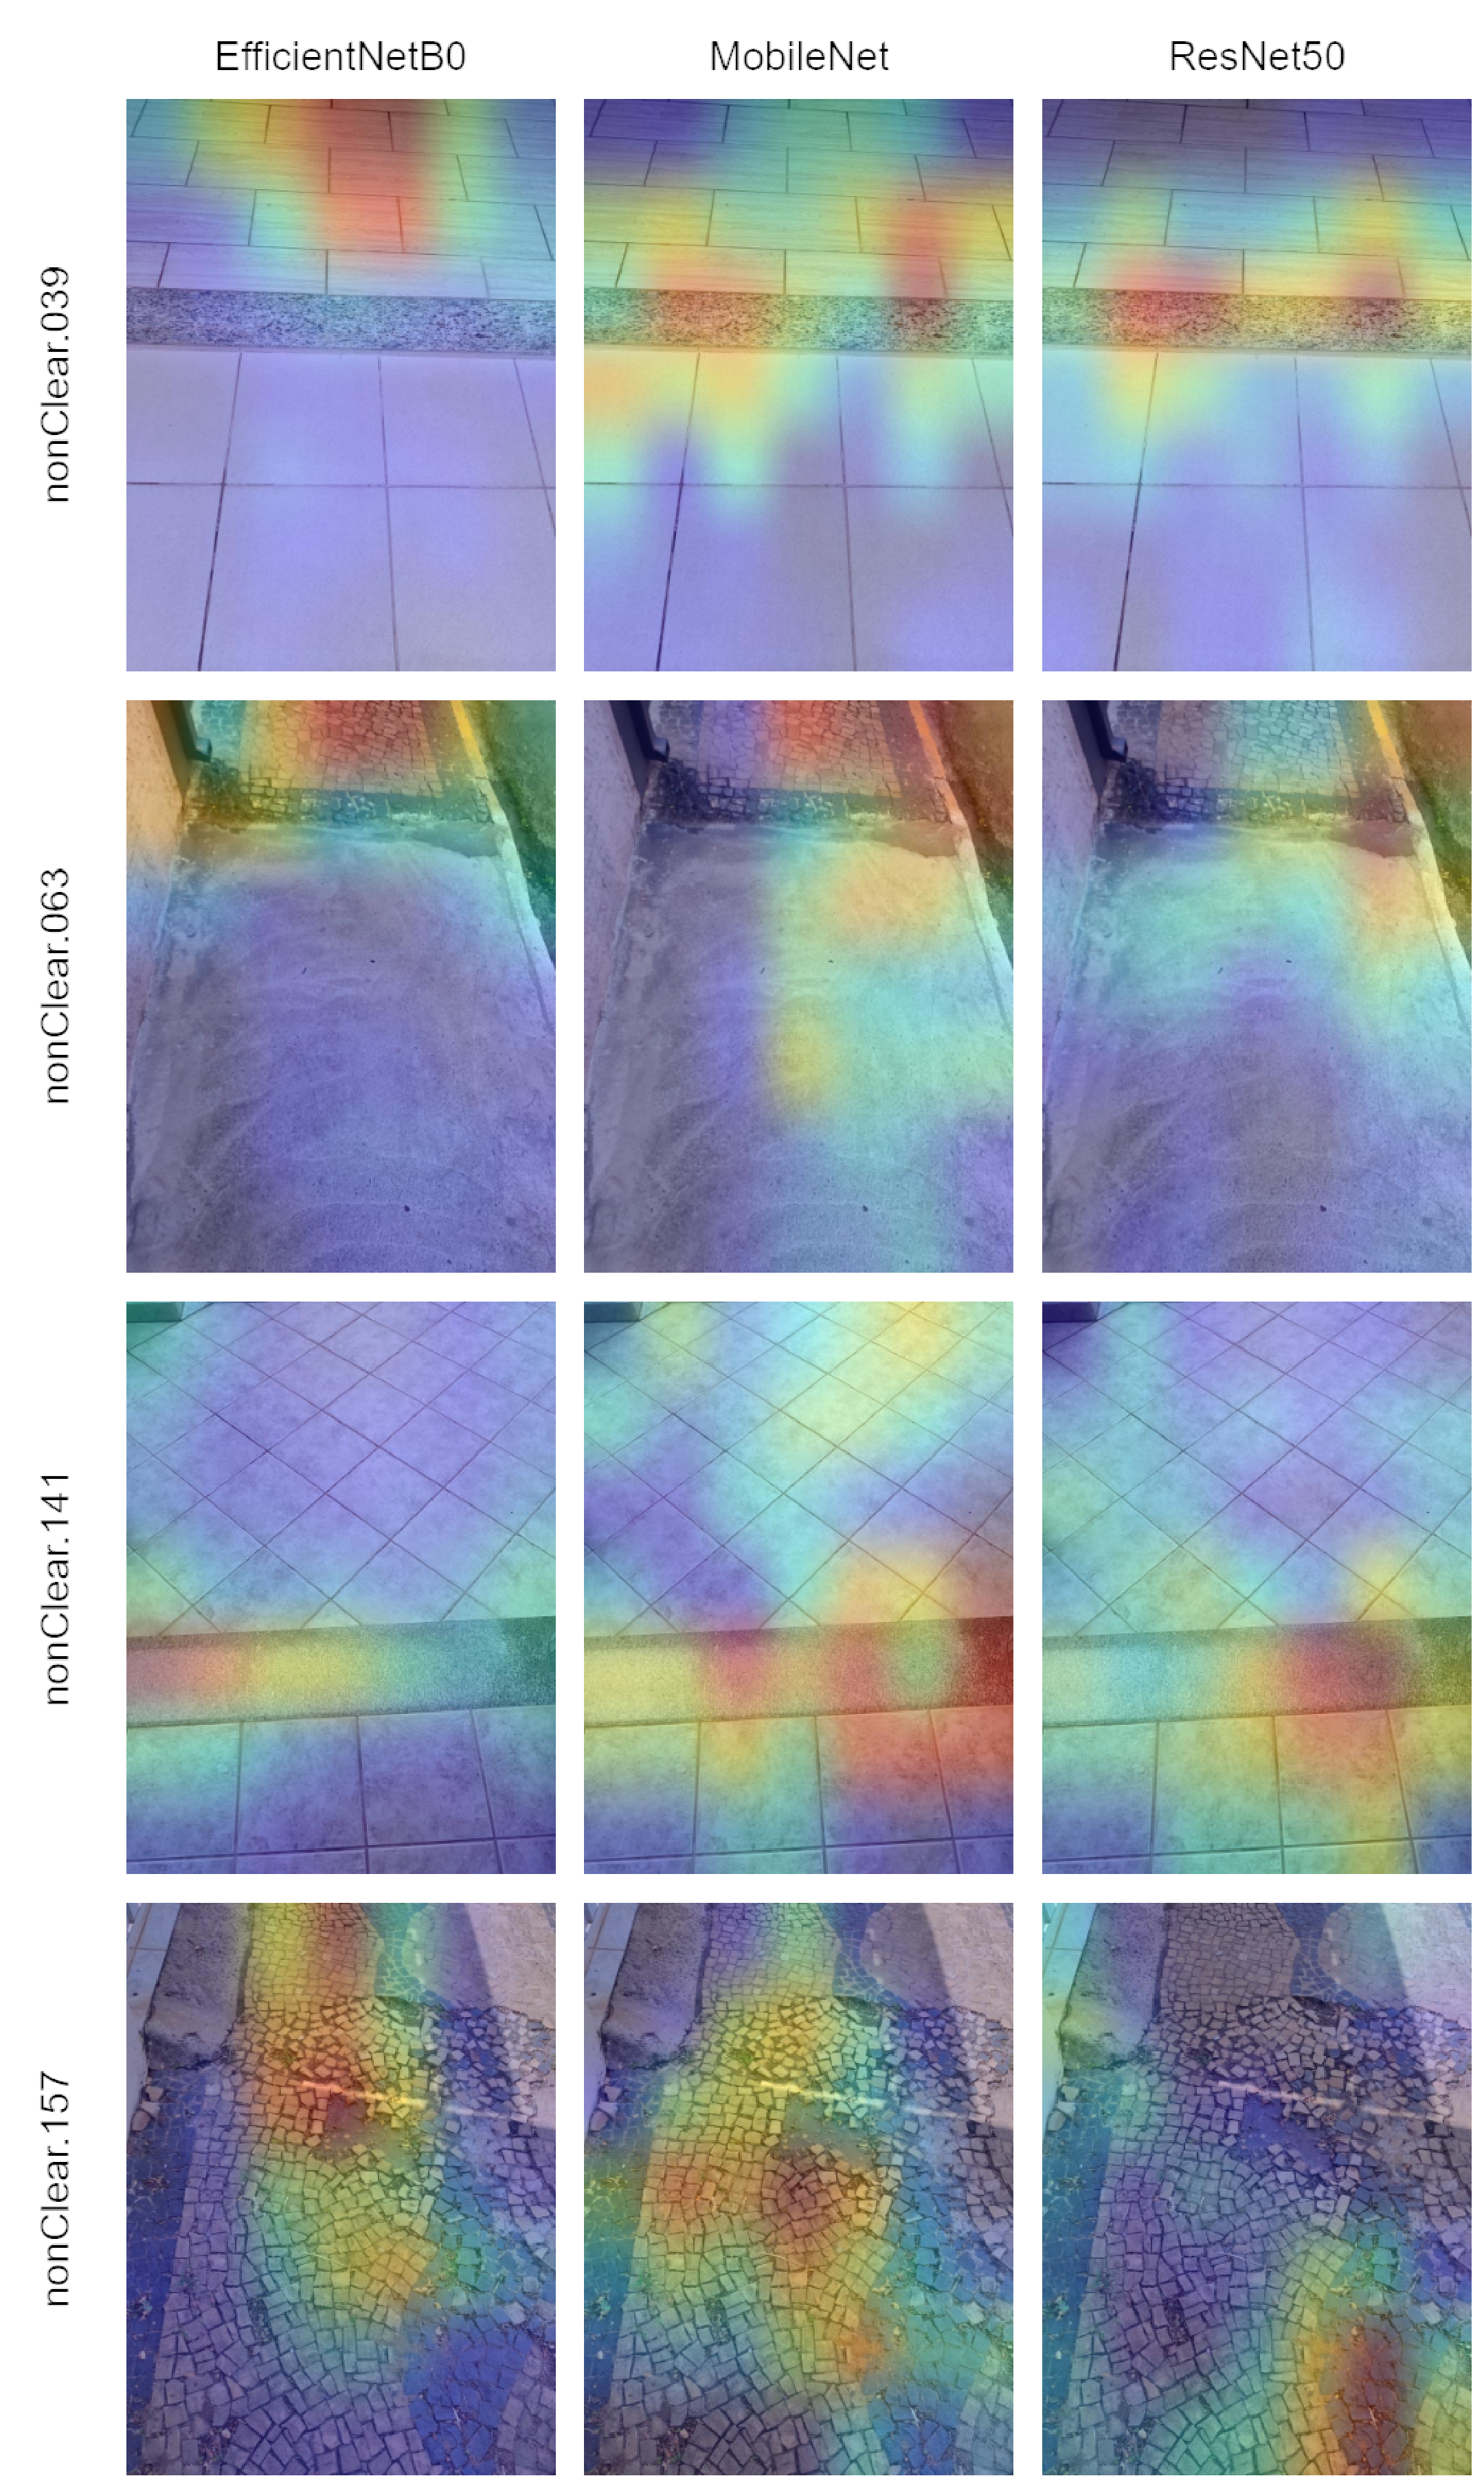
\includegraphics[height=0.8\textheight]{figHeatmap_obstacle_4.eps}
	\caption{CNN Activation Heatmap for Obstructed Path Images with Errors in All Four Approaches.}
	\label{fig:Heatmap_obstacle_4}
\end{figure}

In the images shown in Fig.~\ref{fig:Heatmap_clean_4} (path without obstacles), it appears that the CNNs were activated by changes in ground texture or by the absence of paint on a pedestrian crossing, which ended up being characterized as an obstacle, leading to a classification error. In Fig.~\ref{fig:Heatmap_obstacle_4}, the same phenomenon occurs: the heat areas seem to emphasize changes in texture.

Among the images with 3 errors, some examples of images depicting paths without obstacles can be seen in Fig.~\ref{fig:Heatmap_clean_3}.

\begin{figure}[h!]
	\centering
	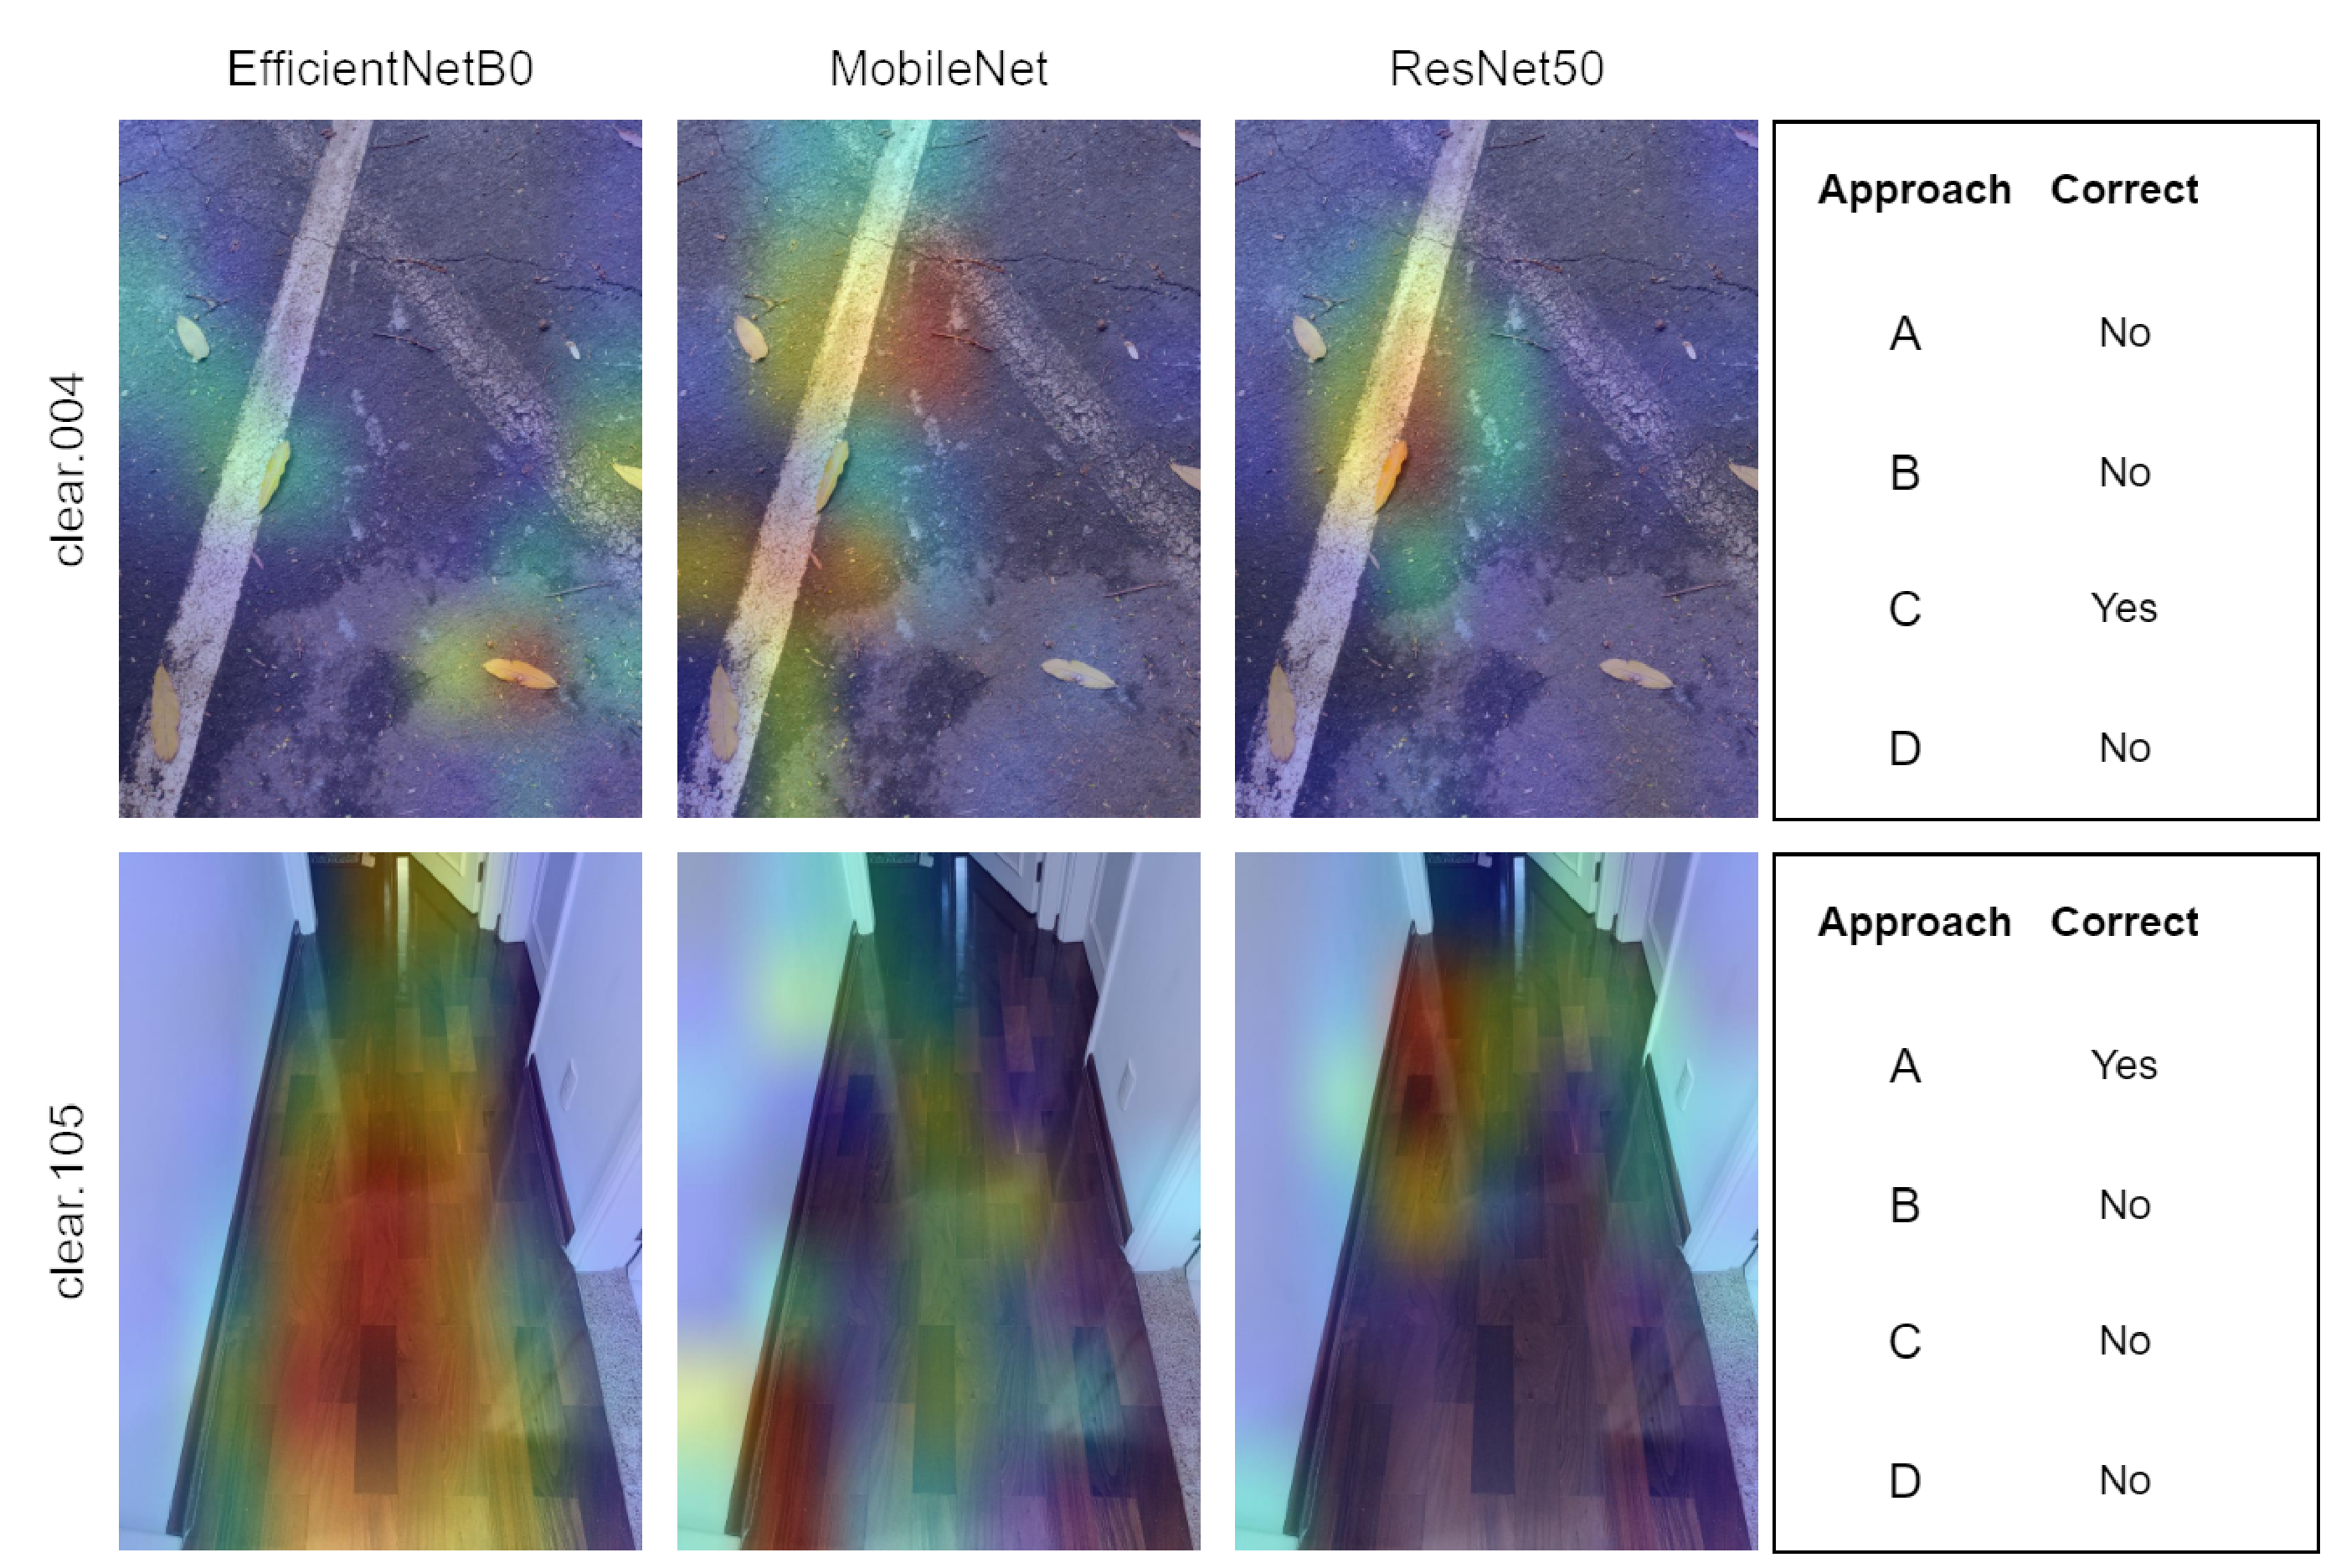
\includegraphics[height=0.45\textheight]{figHeatmap_clean_3.eps}
	\caption{CNN Activation Heatmap for Path Without Obstacles Images with Errors in Three of the Four Approaches.} \label{fig:Heatmap_clean_3}
\end{figure}

Apparently, in the image clear.004, there was a focus by the CNNs on the leaves scattered on the ground, and in the image clear.105, especially in the CNN EfficientNetB0, there was an emphasis on the change in the floor pattern, but the heatmap was more defined along the entire corridor path, which did not occur with the other approaches.

In Fig.~\ref{fig:Heatmap_obstacle_3}, there are examples of images where at least three approaches made incorrect predictions; these images represent paths with obstacles.

\begin{figure}[h!]
	\centering
	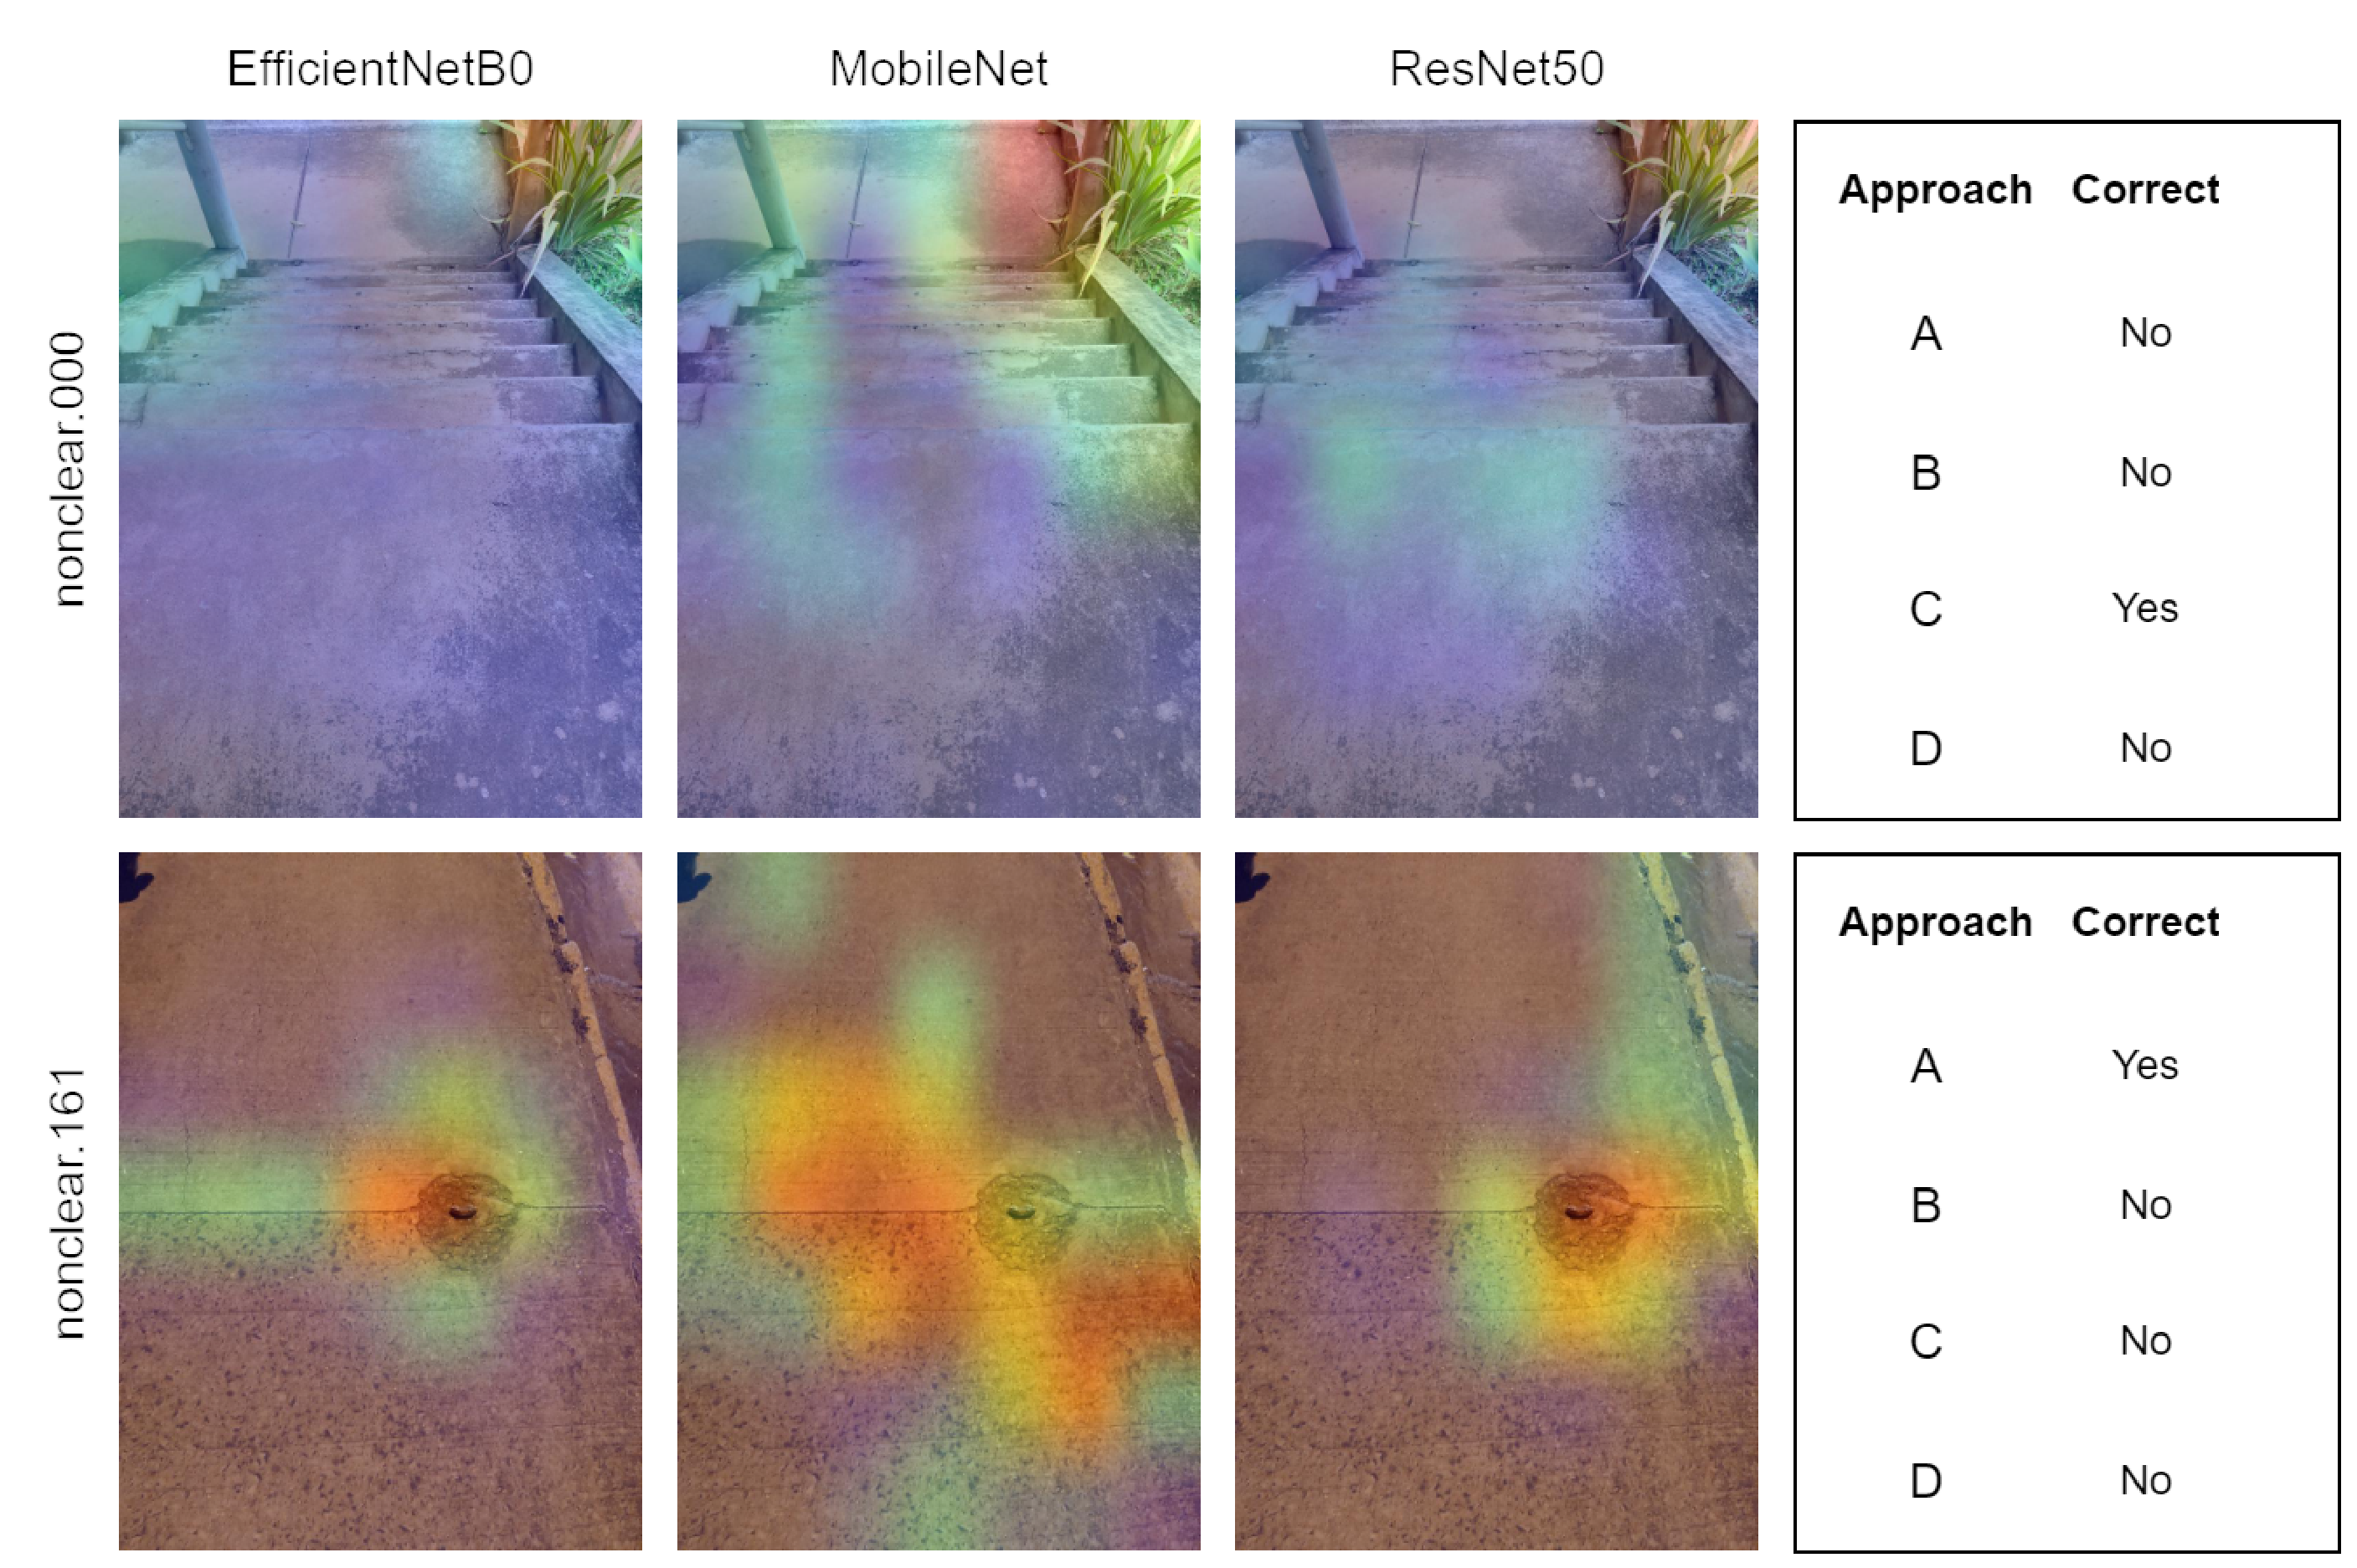
\includegraphics[height=0.45\textheight]{figHeatmap_obstacle_3.eps}
	\caption{CNN Activation Heatmap for Obstructed Path Images with Errors in Three of the Four Approaches.} \label{fig:Heatmap_obstacle_3}
\end{figure}

In the image nonclear.000, the CNNs did not characterize the importance of the main obstacle, which is a staircase, but rather focused on a plant in the garden that does not necessarily represent a problem for the mobility of visually impaired individuals. In the image nonclear.161, there is a more precise focus by the CNN EfficientNetB0 on the obstacle, which is a small hole with the remainder of an iron pipe from a removed post, while the ResNet50 also maintains some focus on the obstacle and the MobileNet spreads its heat zone across the sidewalk.

Many images with incorrect classification are related to markings painted on the ground or to traffic signs: the approaches under study characterize these markings as obstacles. A total of 27 images were identified that characterize paths without obstacles with ground signage; among these images, the error rate was 59.29\%, meaning 16 images were incorrectly classified by at least one of the studied approaches. This issue is illustrated in Fig.~\ref{fig:Heatmap_clean_traffic}, where CNN activations focus on traffic markings. 

\begin{figure}
	\centering
	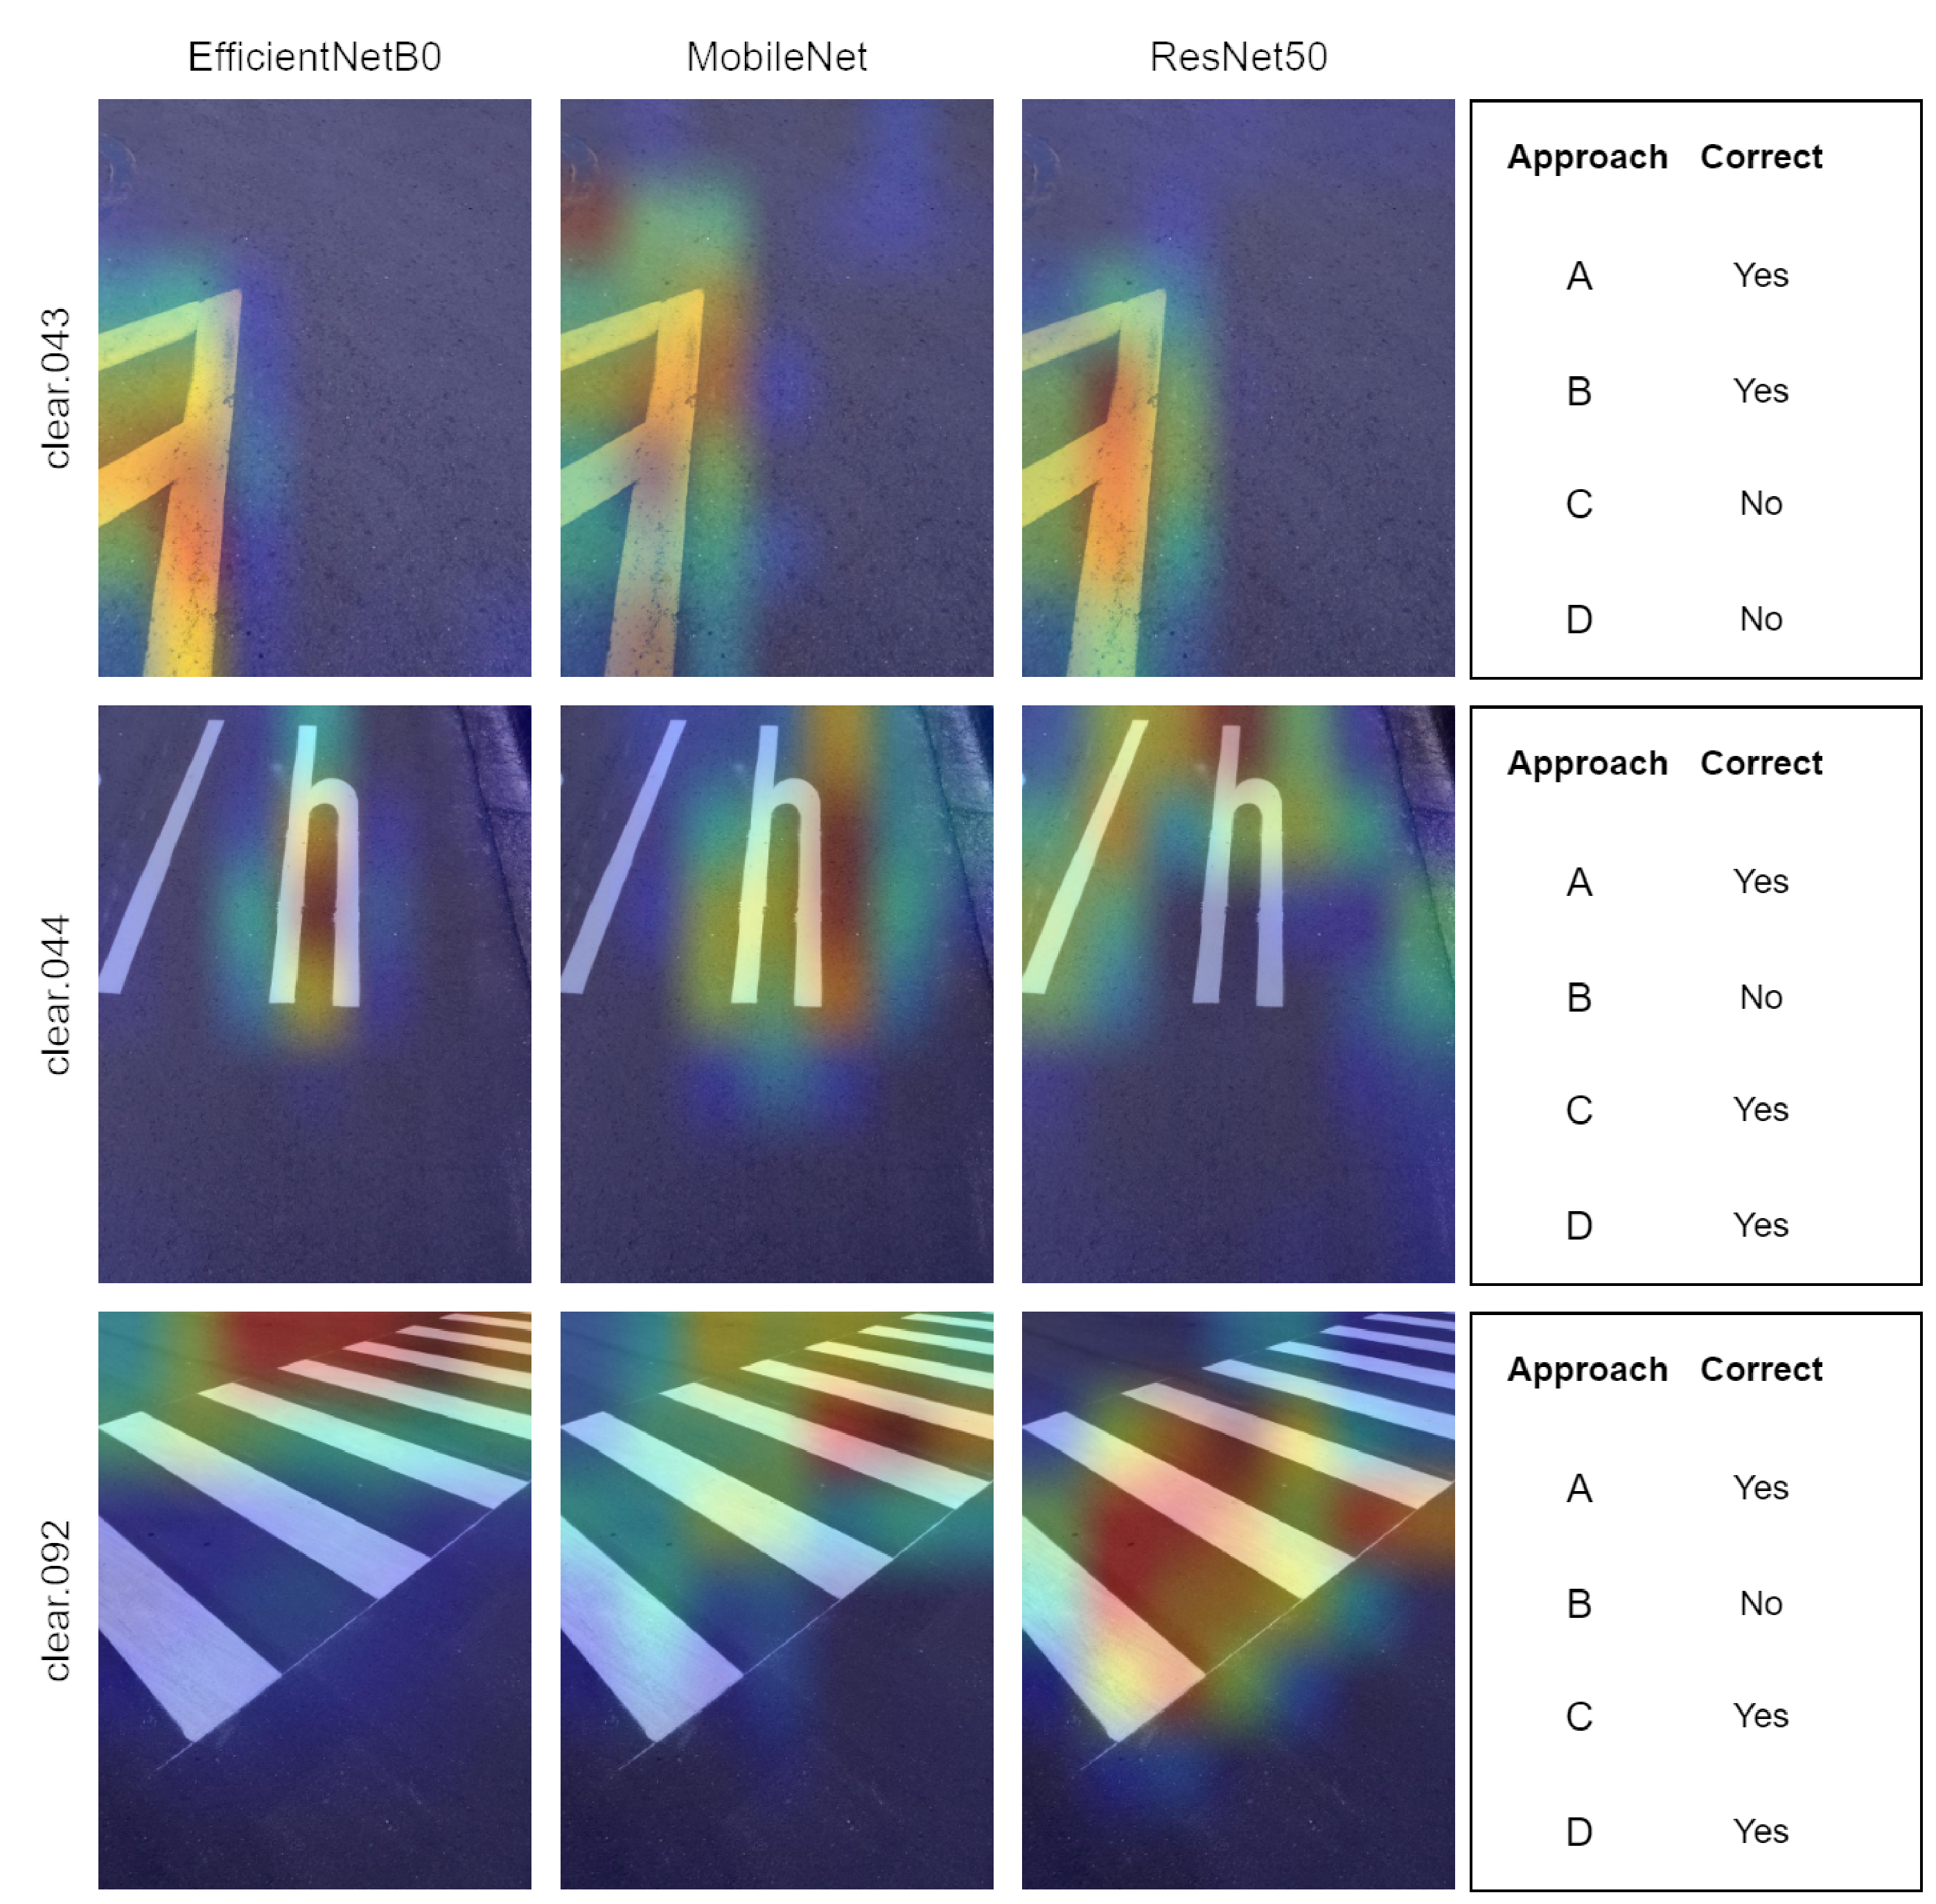
\includegraphics[height=0.6\textheight]{figHeatmap_clean_traffic.eps}
	\caption{CNN Activation Heatmap for Clean Path Images with Ground Traffic Signage.} \label{fig:Heatmap_clean_traffic}
\end{figure}

The focus of the CNN activations concentrates on ground signage, which does not represent an obstacle to visually impaired individuals. In Fig.~\ref{fig:Heatmap_obstacle_traffic}, images with obstacles are observed; in both displayed images, the curb edge is presented as an obstacle to visually impaired individuals. In the image nonclear.033, although all approaches had their predictions correct, the focus of activation for CNNs EfficientNetB0 to a greater degree, and MobileNet, was on the ground signage, and only the CNN ResNet50 focused on the curb edge. Likely, the correct classification provided by the approaches was based on feature extraction that emphasizes traffic signage and not the real obstacle, which is the curb edge.

\begin{figure}
	\centering
	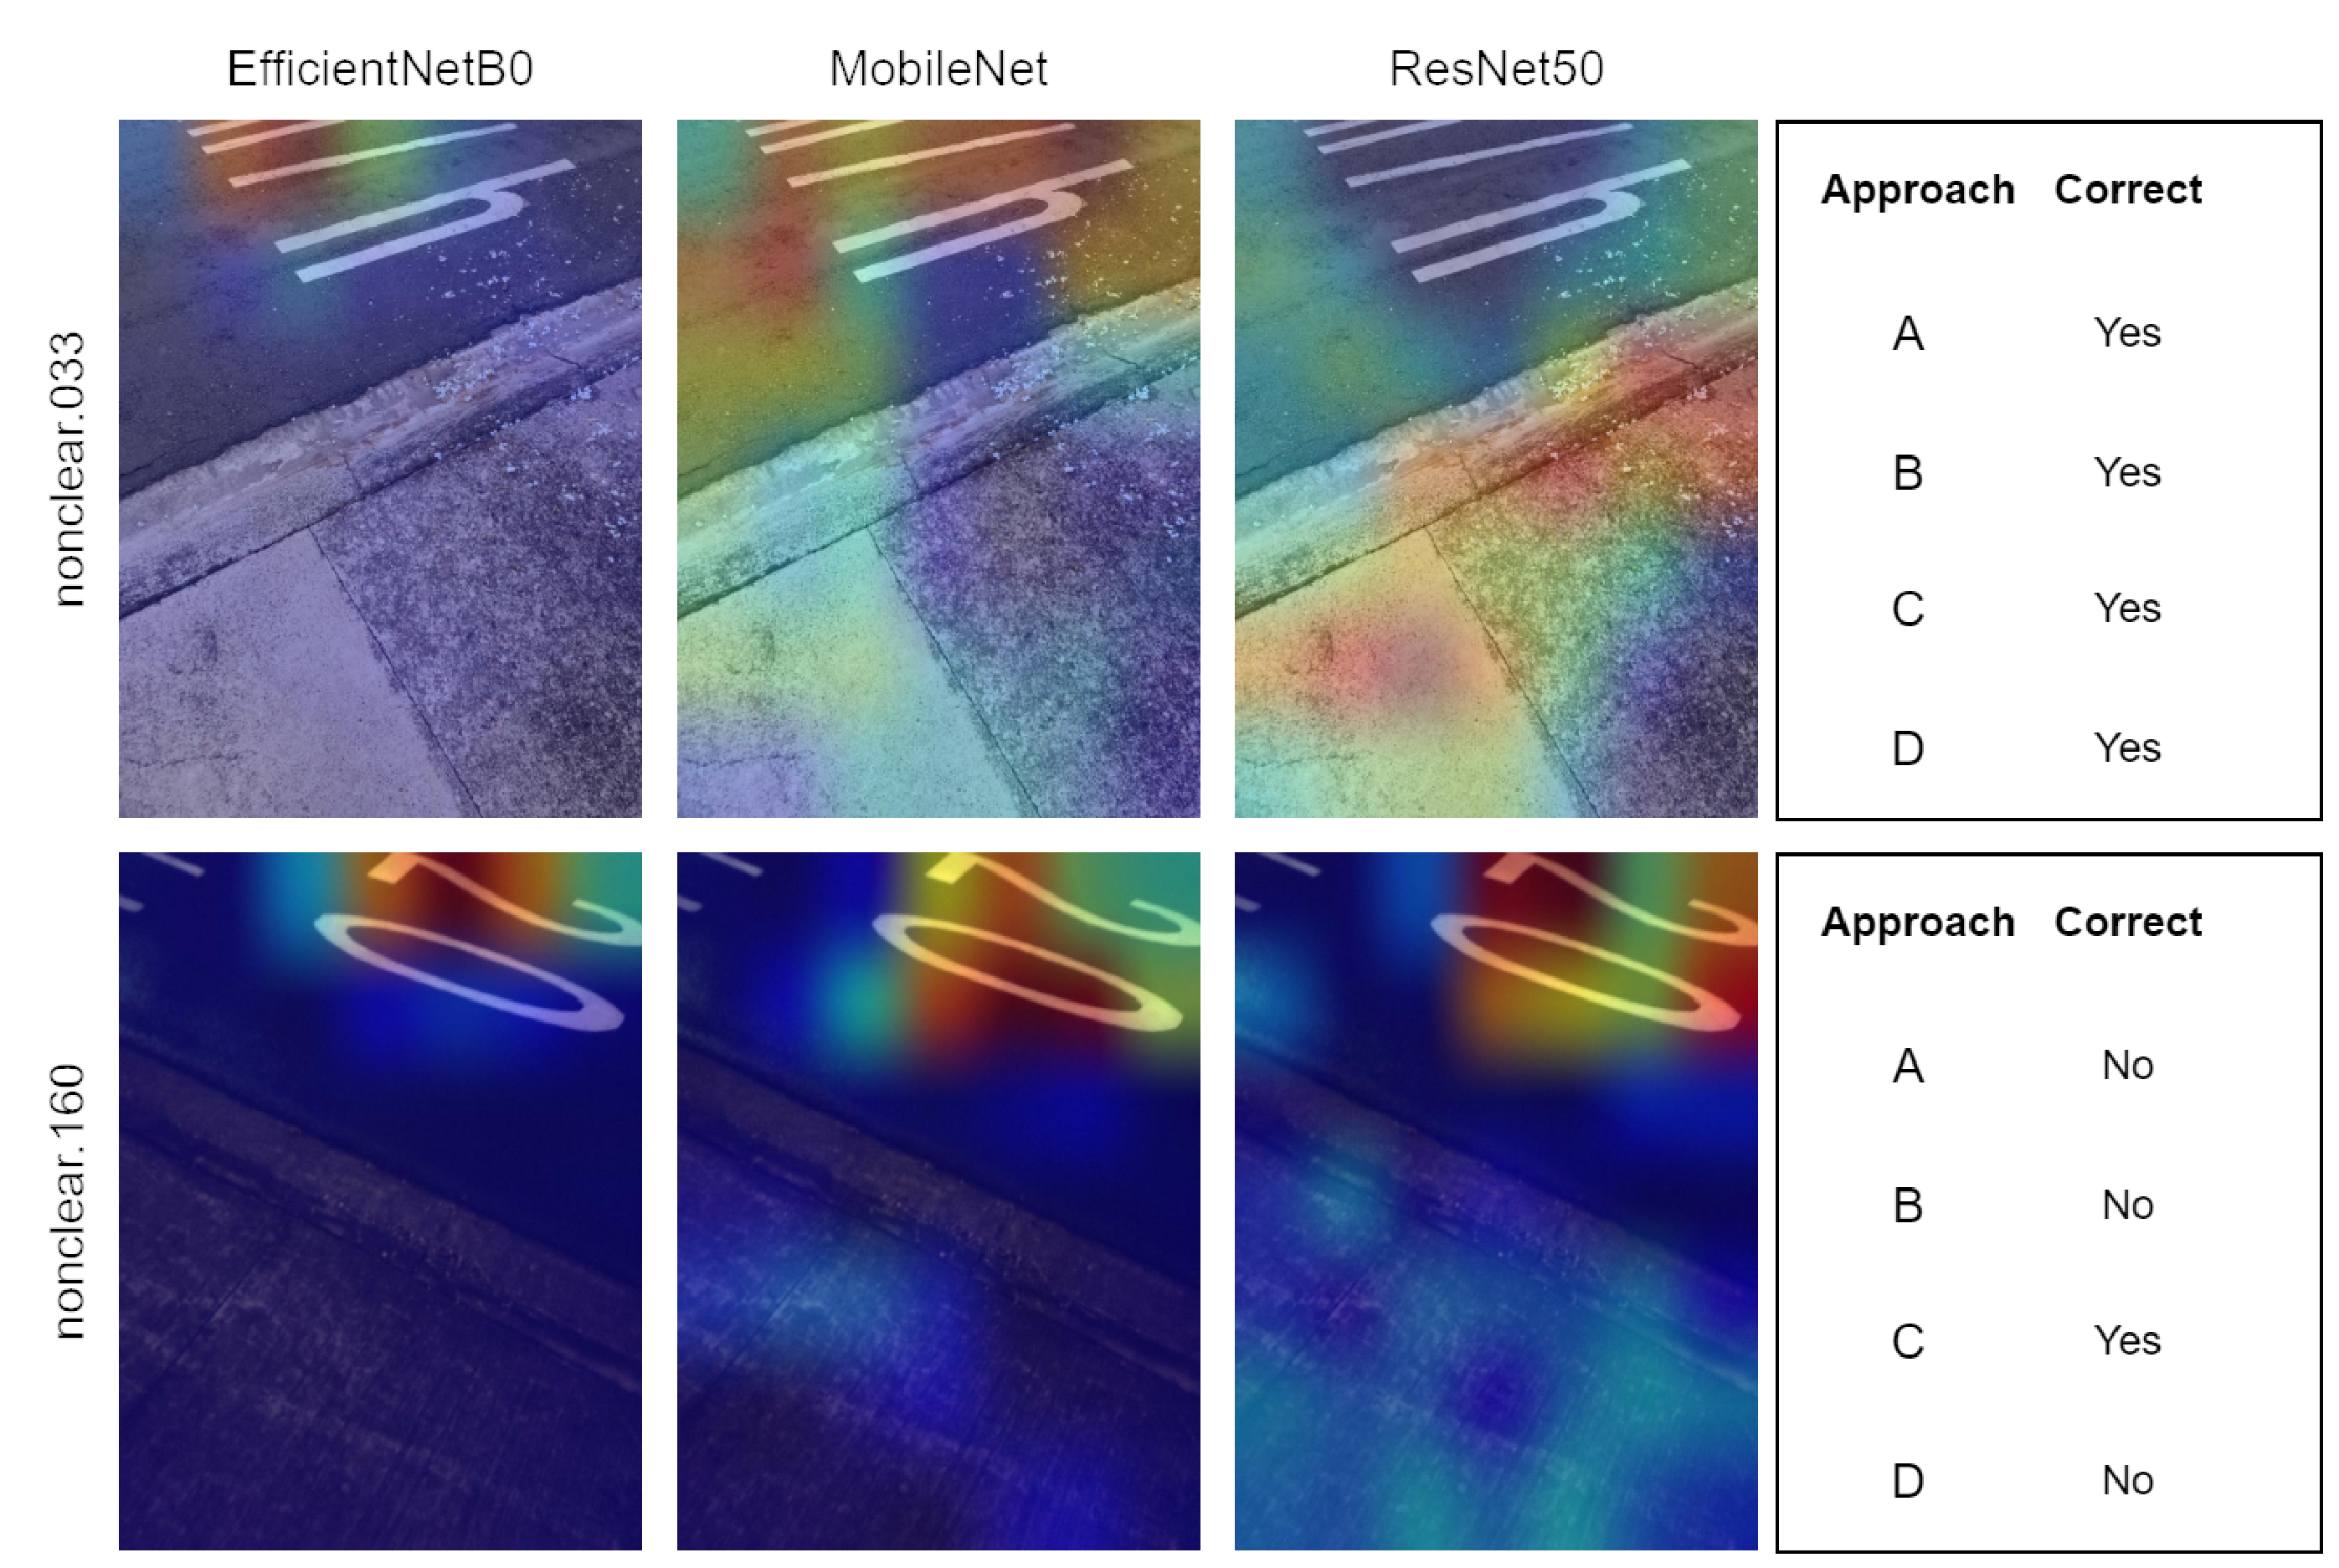
\includegraphics[height=0.45\textheight]{figHeatmap_obstacle_traffic.eps}
	\caption{CNN Activation Heatmap for Obstructed Path Images with Ground Traffic Signage.} \label{fig:Heatmap_obstacle_traffic}
\end{figure}

In the image nonclear.160 (Fig.~\ref{fig:Heatmap_obstacle_traffic}), the CNN ResNet50 demonstrates a wider spread of attention points, but still focusing on traffic signage, and the CNNs EfficientNetB0 and MobileNet have activation points strongly related to traffic signage, again not noticing the curb edge.

The performance of the proposed approaches was assessed in relation to images featuring traffic signage, which can be viewed in Table~\ref{tab:model_accuracy_comparison}. Approach A did not show much fluctuation in accuracy compared to the average observed in the other two tests conducted. In approach C, an improvement in accuracy was observed compared to the individual test with all images and a decrease compared to the test with cross-validation (10-fold). In approaches B and D, a significant drop in accuracy was noted in the test with images featuring ground signage. This fact raises questions about whether the process of dimensionality reduction causes the loss of important information for the correct prediction of this type of image.


\begin{table}[h!]
	\caption{Accuracy Comparison of Proposed Models Using LOOCV for Ground Signage Images, General LOOCV, and 10-fold Cross-Validation}
	\label{tab:model_accuracy_comparison}
	\centering
	\resizebox{\textwidth}{!}{%
		\begin{tabular}{|l|c|c|c|}
			\hline
			\textbf{Proposed} & \textbf{LOOCV Accuracy} & \textbf{LOOCV} & \textbf{10-fold} \\
			\textbf{Model} & \textbf{(Ground Signage Images)} & \textbf{Accuracy} & \textbf{Accuracy} \\
			
			\hline
			\textbf{Approach A} & \textbf{0.9259} & \textbf{0.9474} & \textbf{0.9412} \\
			Approach B & 0.4815 & 0.8713 & 0.9421 \\
			Approach C & 0.8888 & 0.8421 & 0.9559 \\
			Approach D & 0.7037 & 0.8509 & 0.9278 \\
			\hline
		\end{tabular}
	}
\end{table}

Regarding the images without classification errors, a common characteristic is that these images depict everyday objects that are certainly included in the ImageNet database. Thus, due to the transfer learning applied to the CNNs used in this work, it likely facilitates the identification process, as evidenced by the heat zone always being on the objects in Fig.~\ref{fig:Heatmap_noerror}.

\begin{figure}
	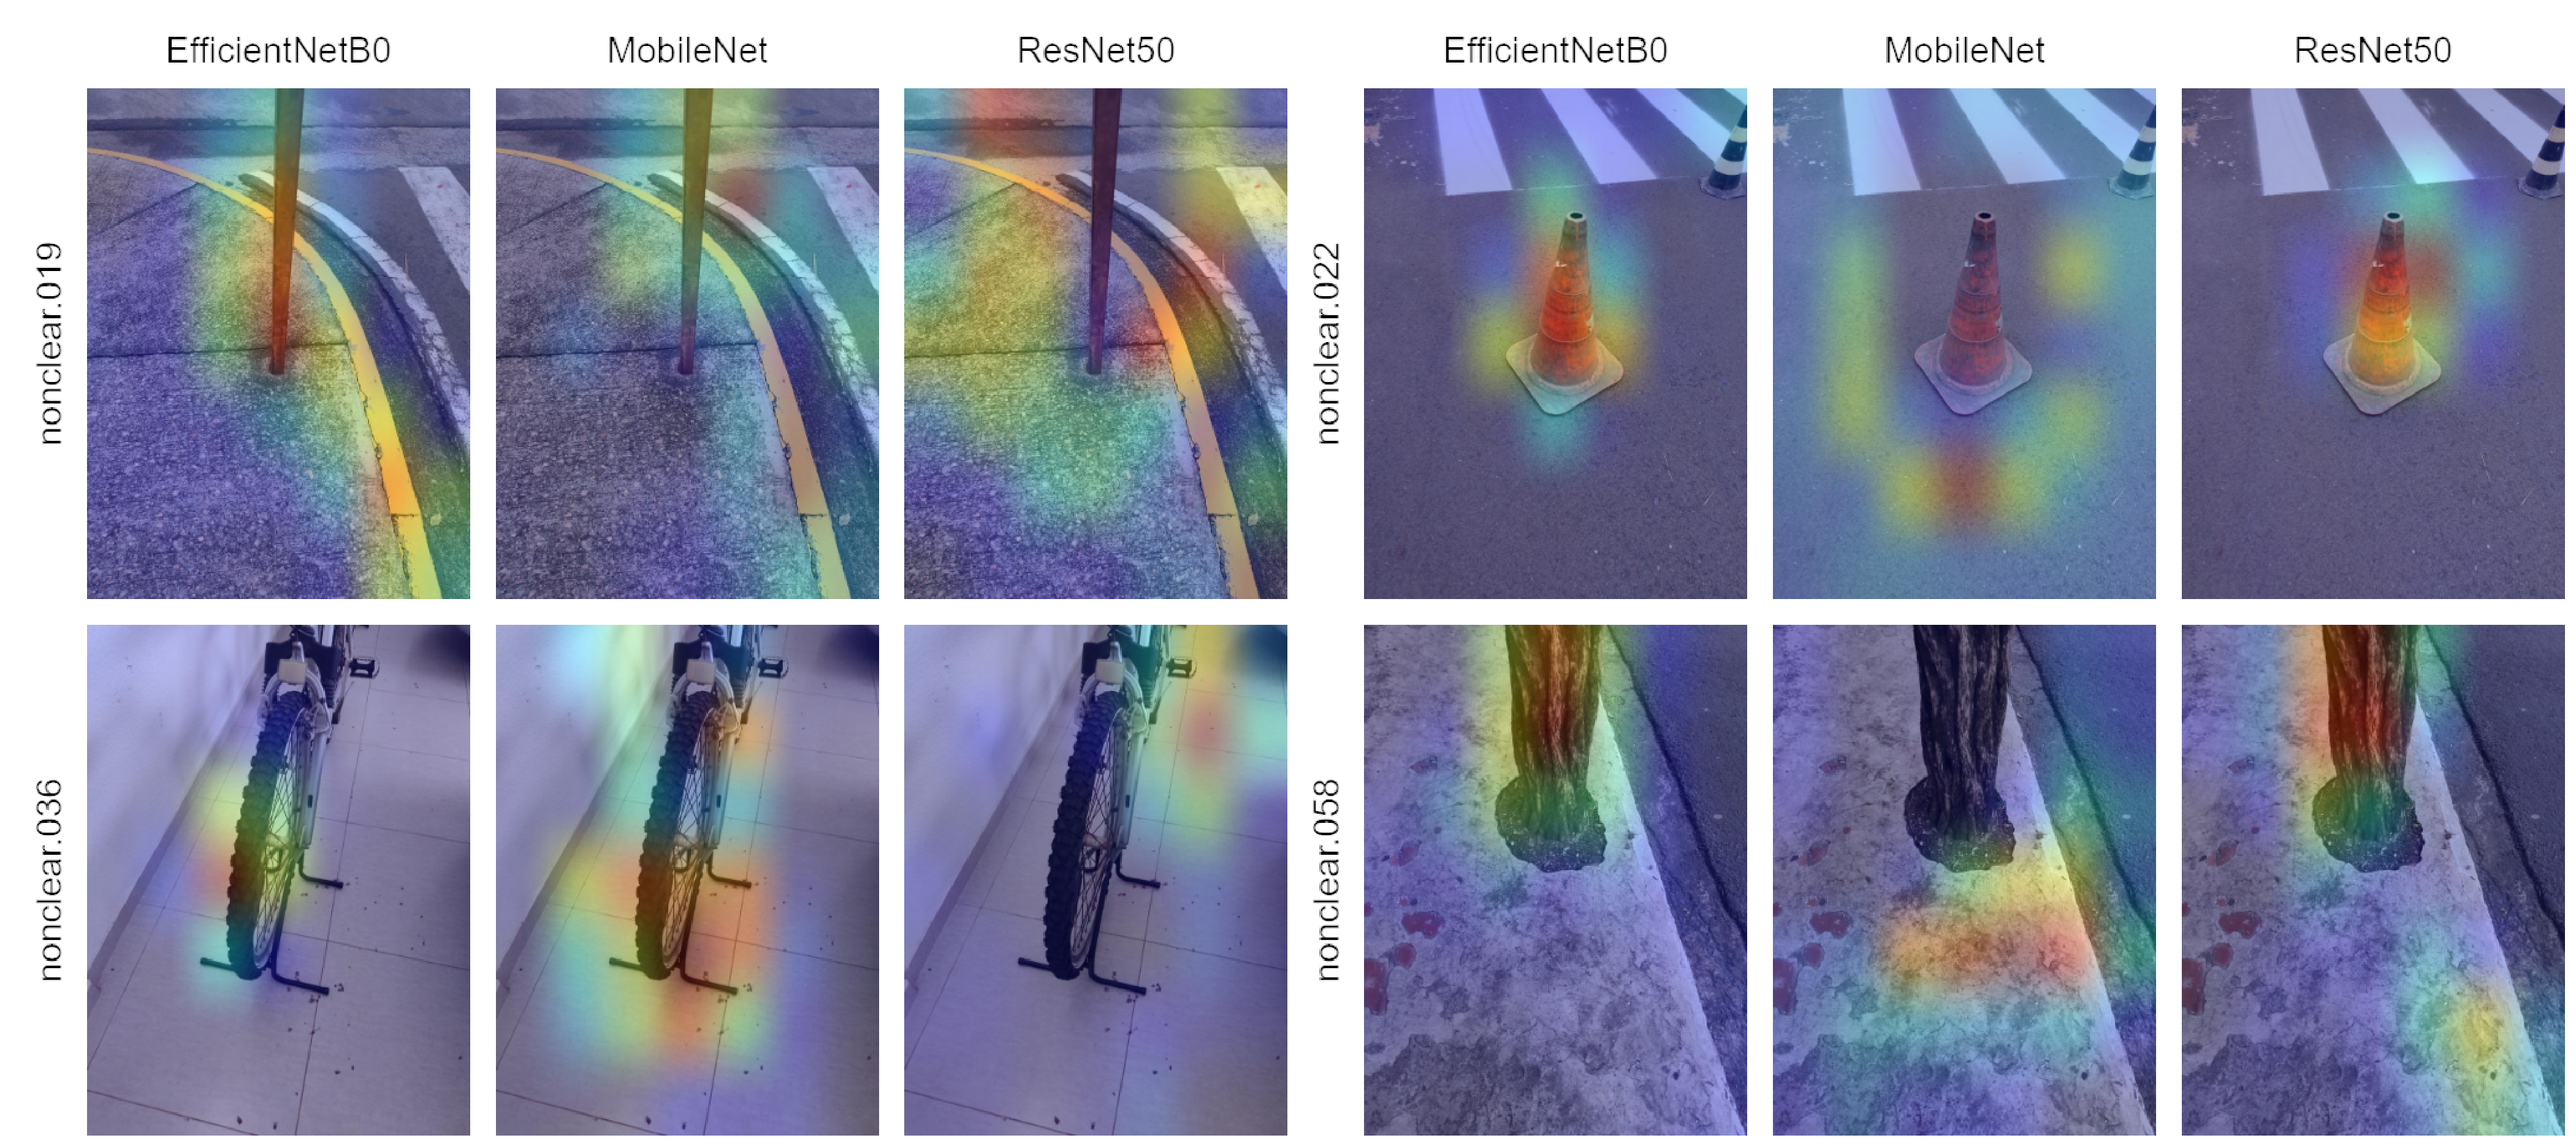
\includegraphics[width=\textwidth]{figHeatmap_no_error.eps}
	\caption{CNN Activation Heatmap for Image with No Classification Error.} \label{fig:Heatmap_noerror}
\end{figure}

If we perform a comparison with the study published by Breve \cite{breve2023}, where the aim was to optimize the performance of CNNs for classification within the image dataset, it can be observed that the best performance was achieved in a scenario of six instances of EfficientNetB4 combined with six instances of EfficientNetB0, with fine-tuning, and six instances of the CNN MobileNet, which were used as feature extractors. This approach from Breve's study \cite{breve2023} resulted in an accuracy of 0.9655. In comparison with this study, the approach with the highest accuracy achieved 0.9559, and the most stable across all studied situations achieved a best result of an accuracy of 0.9474. It should be emphasized that in this study, the CNNs were used without any alterations to their structure, thus eliminating the need for training and solely utilizing transfer learning from the ImageNet database.

\section*{Conclusion}
This study explored the use of 22 CNN architectures combined with dimensionality reduction and supervised classification for the detection of obstacles in environments navigated by visually impaired individuals. The models, applied without any retraining, showed competitive accuracy compared to fine-tuned alternatives. The best-performing model reached 0.9559 accuracy, and the most stable configuration across tests achieved 0.9474. These results demonstrate that systems based exclusively on transfer learning can achieve high performance without significant computational costs. However, limitations were observed in interpreting floor signage, indicating potential for improvement through attention mechanisms or hybrid semantic segmentation. This reinforces the feasibility of lightweight, real-time solutions deployable on mobile devices.

%% The Appendices part is started with the command \appendix;
%% appendix sections are then done as normal sections
%% \appendix

%% \section{}
%% \label{}

%% If you have bibdatabase file and want bibtex to generate the
%% bibitems, please use
%%
%%  \bibliographystyle{elsarticle-num} 
%%  \bibliography{<your bibdatabase>}

%% else use the following coding to input the bibitems directly in the
%% TeX file.

\begin{thebibliography}{00}

%% \bibitem{label}
%% Text of bibliographic item

\bibitem{who2022}
WHO – World Health Organization. Blindness and vision impairment [Internet], 14 October 2021. World Health Organization (WHO), Geneva, Switzerland, 2018. \url{https://www.who.int/news-room/fact-sheets/detail/blindness-and-visual-impairment}. Last acessed 2 jun. 2022.

\bibitem{bourne2017}
Bourne, S. R. F. et al. Magnitude, temporal trends, and projections of the global prevalence of blindness and distance and near vision impairment: a systematic review and meta-analysis. The Lancet Global Health, v. 5, n. 9, pp. e888--e897, August 2, 2017. 10 p.

\bibitem{onu2019}
ONU. World Report on vision. Overview, 8 October 2019. \url{https://www.who.int/publications/i/item/world-report-on-vision}. Last acessed 5 nov 2020. United Nations, Geneva, Switzerland, 2019.

\bibitem{bourne2020}
Bourne, J. A. et al. Trends in prevalence of blindness and distance and near vision impairment over 30 years and contribution to the global burden of disease in 2020. SSRN Electronic Journal, January 2020.

\bibitem{islam2019}
Islam, M.M; Sadi, M.S; Zamli, K.Z; Ahmed, M.M. Devoloping walking assistants for visually impaired people: A review. IEEE Sensors Journal v.19 n. 8, pp. 2814--2828 (2019). \url{https//doi.org/10.1109/JSEN.2018.2890423}.

\bibitem{mandia2023}
Mandia, S., Kumar, A., Verma, K., Deegwal, J.K.: Vision-based assistive systems for visually impaired people: A review. In: Tiwari, M., Ismail, Y., Verma, K.; Garg, A.K. (eds.) Optical and Wireless Technologies. pp. 163-172. Springer Nature Singapore, Singapore (2023)

\bibitem{budrionis2022}
Budrionis, A., Plikynas, D., Daniusis, P., Indrulionis, A.: Smartphonebased computer vision travelling aids for blind and visually impaired individuals: A systematic review. Assistive Technology \textbf{34}(2), pp.178--194 (2022). \url{https://doi.org/10.1080/10400435.2020.1743381}.

\bibitem{kuriakose2021}
Kuriakose, B., Shrestha, R., Sandnes, F.E.: Scenerecog: A deep learning scene recognition model for assisting blind and visually impaired navigate using smartphones. In: 2021 IEEE International Conference on Systems, Man, and Cybernetics (SMC). pp. 2464-2470 (2021). \url{https://doi.org/10.1109/SMC52423.2021.9658913}

\bibitem{cardillo2019}
Cardillo, E., Caddemi, A.: Insight on electronic travel aids for visually impaired people: A review on the electromagnetic technology. Electronics \textbf{8}(11), 1281 (2019)

\bibitem{bai2019}
Bai, J., Liu, Z., Lin, Y., Li, Y., Lian, S., Liu, D.:Wearable travel aid for environment perception and navigation of visually impaired people. Electronics \textbf{8}(6), 697 (2019)

\bibitem{jiang2019}
Jiang, B., Yang, J., Lv, Z., Song, H.: Wearable vision assistance system based on binocular sensors for visually impaired users. IEEE Internet of Things Journal \textbf{6}(2), pp.1375--1383 (April 2019). \url{https://doi.org/10.1109/JIOT.2018.2842229}

\bibitem{joe2019}
Joe Louis Paul, I., Sasirekha, S., Mohanavalli, S., Jayashree, C., Moohana Priya, P., Monika, K.: Smart eye for visually impaired-an aid to help the blind people. In: 2019 International Conference on Computational Intelligence in Data Science (ICCIDS). pp. 1--5 (2019). \url{https://doi.org/10.1109/ICCIDS.2019.8862066}

\bibitem{hoang2017}
Hoang, V.N., Nguyen, T.H., Le, T.L., Tran, T.H., Vuong, T.P., Vuillerme, N.: Obstacle detection and warning system for visually impaired people based on electrode matrix and mobile kinect. Vietnam Journal of Computer Science \textbf{4}(2), pp.71--83 (May 2017). \url{https://doi.org/10.1007/s40595-016-0075-z}

\bibitem{tapu2017}
Tapu, R., Mocanu, B., Zaharia, T.: Deep-see: Joint object detection, tracking and recognition with application to visually impaired navigational assistance. Sensors \textbf{17}(11), 2473 (2017)

\bibitem{saffoury2016}
Saffoury, R., Blank, P., Sessner, J., Groh, B.H., Martindale, C.F., Dorschky, E., Franke, J., Eskofier, B.M.: Blind path obstacle detector using smartphone camera and line laser emitter. In: 2016 1st International Conference on Technology and Innovation in Sports, Health and Wellbeing (TISHW). pp. 1--7. IEEE (2016)

\bibitem{poggi2016}
Poggi, M., Mattoccia, S.: A wearable mobility aid for the visually impaired based on embedded 3d vision and deep learning. In: 2016 IEEE Symposium on Computers and Communication (ISCC). pp. 208--213. IEEE (2016)

\bibitem{lakde2015}
Lakde, C.K., Prasad, P.S.: Review paper on navigation system for visually impaired people. International Journal of Advanced Research in Computer and Communication Engineering \textbf{4}(1) (2015)

\bibitem{poggi2015}
Poggi, M., Nanni, L., Mattoccia, S.: Crosswalk recognition through point-cloud processing and deep-learning suited to a wearable mobility aid for the visually impaired. In: International Conference on Image Analysis and Processing. pp. 282--289. Springer (2015)

\bibitem{rizzo2017}
Rizzo, J.R., Pan, Y., Hudson, T., Wong, E.K., Fang, Y.: Sensor fusion for ecologically valid obstacle identification: Building a comprehensive assistive technology platform for the visually impaired. In: 2017 7th International Conference on Modeling, Simulation, and Applied Optimization (ICMSAO). pp. 1-5. IEEE (2017)

\bibitem{lin2017}
Lin, B.S., Lee, C.C., Chiang, P.Y.: Simple smartphone-based guiding system for visually impaired people. Sensors textbf{17}(6), 1371 (2017)

\bibitem{lecun2015}
LeCun, Y., Bengio, Y., Hinton, G.: Deep learning. Nature \textbf{521}(7553), 436 (2015)

\bibitem{goodfellow2016}
Goodfellow, I., Bengio, Y., Courville, A.: Deep learning. MIT press (2016)

\bibitem{schmidhuber2015}
Schmidhuber, J.: Deep learning in neural networks: An overview. Neural networks n. 61, pp.85--117 (2015)

\bibitem{breve2020}
Breve, F., Fischer, C.N.: Visually impaired aid using convolutional neural networks, transfer learning, and particle competition and cooperation. In: 2020 International Joint Conference on Neural Networks (IJCNN). pp. 1--8 (2020). \url{https://doi.org/10.1109/IJCNN48605.2020.9207606}

\bibitem{russakovsky2015}
Russakovsky, O., Deng, J., Su, H., Krause, J., Satheesh, S., Ma, S., Huang, Z., Karpathy, A., Khosla, A., Bernstein, M., Berg, A.C., Fei-Fei, L.: ImageNet Large Scale Visual Recognition Challenge. International Journal of Computer Vision (IJCV) \textbf{115}(3), pp.211--252 (2015). \url{https://doi.org/10.1007/s11263-015-0816-y}

\bibitem{sanga2023}
Sanga, G. M.; Polo, J.M.G.; Passerini, J.A.R. Auxílio da Deficientes Visuais utilizando Redes Neurais Convolucionais. In: Anais da V Semana Integrada de Estudos – FEF, \textbf{1}(1), pp. 32 (2023). \url{https://fefsisweb.fef.br:8070/sie/issue/view/fefsisweb.fef.br}.

\bibitem{breve2023}
Breve, F. (2023). Convolutional Neural Networks and Ensembles for Visually Impaired Aid. In: Gervasi, O., et al. Computational Science and Its Applications – ICCSA 2023. ICCSA 2023. Lecture Notes in Computer Science, vol 13956. Springer, Cham. \url{https://doi.org/10.1007/978-3-031-36805-9\_34}

\bibitem{tapu2013}
Tapu, R., Mocanu, B., Bursuc, A., Zaharia, T.: A smartphone-based obstacle detection and classification system for assisting visually impaired people. In: The IEEE International Conference on Computer Vision (ICCV) Workshops (June 2013)

\bibitem{kumar2015}
Kumar, R., Meher, S.: A novel method for visually impaired using object recognition. In: 2015 International Conference on Communications and Signal Processing (ICCSP). pp. 0772--0776 (April 2015). \url{https://doi.org/10.1109/ICCSP.2015.7322596}

\bibitem{islam2018}
Islam, M.M., Sadi, M.S.: Path hole detection to assist the visually impaired people in navigation. In: 2018 4th International Conference on Electrical Engineering and Information Communication Technology (iCEEiCT). pp. 268--273 (Sep 2018). \url{https://doi.org/10.1109/CEEICT.2018.8628134}

\bibitem{huang2017}
Huang, G., Liu, Z., van der Maaten, L., Weinberger, K.Q.: Densely connected convolutional networks. In: The IEEE Conference on Computer Vision and Pattern Recognition (CVPR). pp. 4700--4708 (July 2017)

\bibitem{tan2019}
Tan, M., Le, Q.: EfficientNet: Rethinking model scaling for convolutional neural networks. In: Chaudhuri, K., Salakhutdinov, R. (eds.) Proceedings of the 36th International Conference on Machine Learning. Proceedings of Machine Learning Research, vol. 97, pp. 6105--6114. PMLR (09-15 Jun 2019), \url{https://proceedings.mlr.press/v97/tan19a.html}

\bibitem{szegedy2016}
Szegedy, C., Vanhoucke, V., Ioffe, S., Shlens, J., Wojna, Z.: Rethinking the inception architecture for computer vision. In: The IEEE Conference on Computer Vision and Pattern Recognition (CVPR). pp. 2818--2826 (June 2016) 

\bibitem{szegedy2017}
Szegedy, C., Ioffe, S., Vanhoucke, V., Alemi, A.A.: Inception-v4, inception-resnet and the impact of residual connections on learning. In: Thirty-First AAAI conference on artificial intelligence (2017)

\bibitem{howard2017}
Howard, A.G., Zhu, M., Chen, B., Kalenichenko, D., Wang, W., Weyand, T., Andreetto, M., Adam, H.: Mobilenets: Efficient convolutional neural networks for mobile vision applications. arXiv preprint arXiv:1704.04861 (2017)

\bibitem{sandler2018}
Sandler, M., Howard, A., Zhu, M., Zhmoginov, A., Chen, L.C.: Mobilenetv2: Inverted residuals and linear bottlenecks. In: The IEEE Conference on Computer Vision and Pattern Recognition (CVPR). pp. 4510--4520 (June 2018)

\bibitem{zoph2018}
Zoph, B., Vasudevan, V., Shlens, J., Le, Q.V.: Learning transferable architectures for scalable image recognition. In: The IEEE Conference on Computer Vision and Pattern Recognition (CVPR). pp. 8697--8710 (June 2018)

\bibitem{he2016}
He, K., Zhang, X., Ren, S., Sun, J.: Deep residual learning for image recognition. In: The IEEE Conference on Computer Vision and Pattern Recognition (CVPR). pp. 770--778 (June 2016)

\bibitem{zhang2016}
He, K., Zhang, X., Ren, S., Sun, J.: Identity mappings in deep residual networks. In: Leibe, B., Matas, J., Sebe, N., Welling, M. (eds.) Computer Vision ECCV 2016. pp. 630--645. Springer International Publishing, Cham (2016)

\bibitem{simonyan2015}
Simonyan, K., Zisserman, A.: Very deep convolutional networks for large-scale image recognition. pp. 1--14. Computational and Biological Learning Society (2015)

\bibitem{chollet2017}
Chollet, F.: Xception: Deep learning with depthwise separable convolutions. In: 2017 IEEE Conference on Computer Vision and Pattern Recognition (CVPR). pp. 1800--1807 (July 2017). \url{https://doi.org/10.1109/CVPR.2017.195}

\bibitem{jolliffe2002}
Jolliffe, I. T. Principal components analysis. 2nd. ed. Heidelberg, Germany: Springer-Verlag Berlin Heidelberg, 2002. (Springer Series in Statistics SSS)

\bibitem{mcinnes2021}
McInnes, L.; Healy, J.; Melville, J. UMAP: uniform manifold approximation and projection for dimension reduction. [Internet] September 21, 2020. Disponível em: \url{arxiv.org/abs/1802.03426v3} [stat.ML] 18 Sep 2020. Last acessed 10 nov. 2021

\bibitem{kononenko1994}
Kononenko, I. Estimating attributes: analysis and extensions of RELIEF. In: Bergadano, F., DE Raedi, L (eds.) Machine Learning: ECML-94 Lecture notes in Computer Sciences, v. 784, pp. 171--182, Springer, 1 May 1994

\bibitem{priyanka2020}
Priyanka and Kumar, D. Decision tree classifier: a detailed survey. Int. J. Information and Decision Sciences, v. 12, n. 3, pp. 246--269, 2020.

\bibitem{liu2011}
Liu, Q. et al. Feature selection for support vector machines with RBF kernel. Artif Intell Rev. v. 36, pp. 99--115, 2011.

\bibitem{lorena2003}
Lorena, A. C; Carvalho, A. C. P. L. F. Introdução máquinas de vetores de suporte. Relatório Técnico do Instituto de Ciências Matemáticas e de Computação [192]. São Carlos, SP: ICMS-USP, 2003. 66 p.

\bibitem{pereira2013}
Pereira, L. A. d. A. Classificação automática de áreas cafeeiras em imagens de satélites, utilizando redes neurais artificiais. 2013. 83 f. Monografia (Bacharel em Ciência da Computação) – Curso de Ciência da Computação, Universidade Federal de Lavras, Lavras, MG, 2013.

\bibitem{ekstrom2018}
Ekström, M. et al. Logistic regression for clustered data from environmental monitoring programs. Ecological Informatics, Elsevier, v. 43, pp. 165--173, January 2018.

\bibitem{breiman2001}
Breiman, L. Random Forests. Machine Learning, v. 45, n. 1, pp. 5--32, October 2001.

\bibitem{zhu2009}
Zhu, J. et al. Multi-class Adaboost. Statistics and Its Interface, v. 2, n. 3, pp. 349--360, 2009 

\bibitem{gayathri2016}
Gayathri, B. M; Sumathi, C. P. An automated technique using Gaussian Naïve Bayes classifier to classify breast cancer. International Journal of Computer Applications, v. 148, n. 6, pp. 16--21, August 2016.

\bibitem{selvaraju2020}
Selvaraju, R. R. et al. Grad-CAM: visual explanations from deep networks via gradient-based localization. International Journal of Computer Vision, n. 128, pp. 336--359, February 2020.


\end{thebibliography}
\end{document}
\endinput
%%
%% End of file `elsarticle-template-num.tex'.
